\chapter{MATERIAL E MÉTODOS}
\label{cap:materiais-metodos}

Este capítulo descreve os materiais e métodos empregados no
desenvolvimento do sistema proposto. A exposição segue quatro eixos:
o modelo de alerta hidrometeorológico, que define o que é monitorado e
como o nível de alerta é determinado; as fontes externas de dados
meteorológicos que alimentam esse modelo; a plataforma de
\textit{software} que implementa o modelo e disponibiliza seus
resultados; e o protótipo de \textit{hardware} embarcado, responsável
pela coleta dos dados em campo.

Ao final, descreve-se a metodologia dos testes de validação, cujos
resultados são apresentados no \autoref{cap:resultados}.

Conforme orientação da Coordenação de Aperfeiçoamento de Pessoal de
Nível Superior (CAPES) quanto à transparência no uso de ferramentas de
inteligência artificial em trabalhos acadêmicos, registra-se que a
ferramenta de inteligência artificial generativa Claude, desenvolvida
pela Anthropic, foi utilizada como recurso auxiliar neste trabalho.

O uso ocorreu em quatro frentes: (i) depuração do código-fonte, incluindo auxílio na 
análise de trechos de código, identificação de inconsistências, 
elaboração e revisão de funções e estruturas utilizadas no \textit{firmware} embarcado, 
no \textit{backend} e no \textit{frontend} do sistema; (ii) elaboração e revisão
do código dos diagramas do sistema; (iii) apoio à busca e à
conferência de referências bibliográficas; e (iv) revisão textual
deste documento, quanto a clareza, coesão, linguagem acadêmica e
formatação.

As sugestões geradas foram analisadas, testadas e, quando pertinentes,
adaptadas pela autora. As informações extraídas das referências foram
conferidas nas fontes originais. A ferramenta não substituiu a
análise, a validação dos resultados nem as decisões técnicas.

A escolha do modelo de alerta e dos limiares, a partir da literatura
citada, as decisões de arquitetura e implementação, a execução dos
testes, a interpretação dos resultados e as conclusões são de
responsabilidade e autoria da autora.

% =============================================================
\section{Modelo de Alerta Hidrometeorológico}
\label{sec:modelo-risco}
% =============================================================

Em barragens de rejeitos, a ruptura raramente decorre de uma causa
isolada. No levantamento de 147 casos feito por
\citeonline[p.~848]{rico2008mine}, 39\% das rupturas resultaram da
combinação de diferentes fatores. As causas meteorológicas, como
eventos ou períodos de chuva incomum, responderam por 25\% dos casos
no mundo e por 35\% na Europa.

Para escorregamentos induzidos por chuva,
\citeonline{bogaard2018hydrological} propõem separar dois fatores com
escalas de tempo distintas: a umidade antecedente do terreno, que atua
como causa, e a chuva de curto prazo, que atua como gatilho. Com base
nessa ideia, \citeonline{mirus2018developing} desenvolveram limiares
hidrometeorológicos que combinam a saturação do solo medida em campo
com a chuva acumulada em uma janela que inclui as 24 horas seguintes.

O modelo de alerta deste trabalho adota essa estrutura e utiliza três
dados: a saturação relativa do solo ($S$), obtida pelo higrômetro; a
chuva observada nas últimas 48 horas, obtida da API BNDMET; e a chuva
prevista para as próximas 24 horas, obtida da API OpenWeatherMap
(\autoref{sec:fontes-dados}). Com esses dados, o modelo classifica a
condição da estrutura em três níveis: VERDE, AMARELO e VERMELHO.

% -------------------------------------------------------------
\subsection{Saturação Relativa do Solo}
\label{subsec:saturacao}
% -------------------------------------------------------------

A saturação relativa do solo é obtida pela normalização mínimo--máximo
da leitura do higrômetro, adaptada de \citeonline{wicki2020assessing},
conforme a \autoref{eq:saturacao}. Nesses autores, o valor máximo
corresponde ao percentil de 99,9\% da série de umidade; neste
trabalho, ele foi substituído pela leitura de calibração com o solo
saturado.

\begin{equation}
\label{eq:saturacao}
S = \frac{L - L_{\mathrm{seco}}}{L_{\mathrm{sat}} - L_{\mathrm{seco}}}
\end{equation}

Cada variável da \autoref{eq:saturacao} é descrita a seguir:

\begin{itemize}
  \item $S$: saturação relativa do solo, adimensional, de 0 (solo
        seco) a 1 (solo saturado);
  \item $L$: leitura atual do conversor analógico-digital (ADC) do
        higrômetro;
  \item $L_{\mathrm{seco}}$: leitura do ADC com o sensor em solo seco,
        registrada na calibração;
  \item $L_{\mathrm{sat}}$: leitura do ADC com o sensor em solo
        saturado, registrada na calibração.
\end{itemize}

A escala de 0 a 1 segue a definição de saturação de
\citeonline[p.~5]{mirus2018developing}, que dividem a umidade
volumétrica medida pela porosidade, tomada como a máxima umidade
observada no local. Valores calculados fora desse intervalo, causados
por ruído de leitura, são limitados a 0 ou a 1.

O higrômetro resistivo (\autoref{subsec:higrometro}) fornece uma
leitura elétrica, e não a umidade volumétrica. Por isso, $S$ é uma
saturação relativa à calibração do sensor. A expressão vale tanto
para leituras que aumentam quanto para as que diminuem com a umidade,
pois numerador e denominador mudam de sinal juntos.

% -------------------------------------------------------------
\subsection{Chuva Acumulada na Janela de 72 Horas}
\label{subsec:chuva72h}
% -------------------------------------------------------------

A variável meteorológica do modelo é a chuva acumulada em uma janela
de 72 horas, que vai de 48 horas antes até 24 horas depois do instante
de análise. Essa janela foi definida por
\citeonline[p.~5]{mirus2018developing}, que calculam a chuva acumulada
de $t-48$\,h até $t+24$\,h. O valor é obtido pela \autoref{eq:p72}.

\begin{equation}
\label{eq:p72}
P_{72} = P_{48,\mathrm{obs}} + P_{24,\mathrm{prev}}
\end{equation}

Cada variável da \autoref{eq:p72} é descrita a seguir:

\begin{itemize}
  \item $P_{72}$: chuva acumulada na janela de 72 horas, em mm;
  \item $P_{48,\mathrm{obs}}$: chuva observada nas últimas 48 horas,
        em mm, obtida da API BNDMET (\autoref{subsec:bndmet});
  \item $P_{24,\mathrm{prev}}$: chuva prevista para as próximas 24
        horas, em mm, obtida pela soma dos oito blocos de 3 horas do
        \textit{endpoint} \texttt{/forecast} da API OpenWeatherMap
        (\autoref{subsec:owm}).
\end{itemize}

Na formulação original, \citeonline[p.~5]{mirus2018developing} usaram
a chuva medida após o evento como substituta de uma previsão exata.
Neste trabalho, a parcela futura vem de uma previsão real e, por isso,
carrega o erro próprio da previsão meteorológica.

% -------------------------------------------------------------
\subsection{Regra de Decisão do Nível de Alerta}
\label{subsec:regra-decisao}
% -------------------------------------------------------------

O nível de alerta é definido por dois pares de limiares, cada um com
um valor de saturação e um valor de chuva. O nível só sobe quando a
saturação e a chuva acumulada ultrapassam, ao mesmo tempo, os limiares
correspondentes. Essa estrutura segue os limiares hidrometeorológicos
de \citeonline{mirus2018developing}, nos quais o valor de chuva e o de
saturação devem ser superados juntos. A regra é dada pela
\autoref{eq:nivel}.

\begin{equation}
\label{eq:nivel}
N =
\begin{cases}
\text{VERMELHO}, & \text{se } S \geq S_2 \text{ e } P_{72} \geq P_2;\\[2pt]
\text{AMARELO},  & \text{se } S \geq S_1 \text{ e } P_{72} \geq P_1
                   \text{, sem atender ao nível VERMELHO;}\\[2pt]
\text{VERDE},    & \text{nos demais casos.}
\end{cases}
\end{equation}

Cada variável da \autoref{eq:nivel} é descrita a seguir:

\begin{itemize}
  \item $N$: nível de alerta resultante;
  \item $S$: saturação relativa do solo (\autoref{eq:saturacao});
  \item $P_{72}$: chuva acumulada na janela de 72 horas, em mm
        (\autoref{eq:p72});
  \item $S_1$ e $S_2$: limiares de saturação de atenção e de alerta,
        adimensionais;
  \item $P_1$ e $P_2$: limiares de chuva em 72 horas de atenção e de
        alerta, em mm.
\end{itemize}

Os valores de $S_1$, $S_2$, $P_1$ e $P_2$ estão na
\autoref{tab:limiares}. Com dois limiares, formam-se três zonas, que
correspondem ao sistema de alerta duplo descrito por
\citeonline[p.~14]{mirus2018developing} para indicar quando os
escorregamentos são improváveis, possíveis ou prováveis. Neste
trabalho, essas zonas correspondem aos níveis VERDE, AMARELO e
VERMELHO.

Cada nível acende o LED da cor correspondente. No nível VERMELHO, o
\textit{buzzer} também é acionado (\autoref{sec:hardware}).

% -------------------------------------------------------------
\subsection{Limiares Adotados}
\label{subsec:limiares}
% -------------------------------------------------------------

Os limiares de saturação vêm de
\citeonline[p.~9, Tabela~1]{mirus2018developing}. Para a região de
Seattle, os autores obtiveram limiares de saturação entre 0,64,
otimizado pelo ponto ótimo com saturação média de 9 dias, e 0,86,
otimizado pelo \textit{threat score} com saturação média de 1 dia. O
valor inferior foi adotado como limiar de atenção ($S_1$) e o
superior, como limiar de alerta ($S_2$).

Em Portland, os mesmos autores obtiveram 0,70 (ponto ótimo) e 0,75
(\textit{threat score}) \cite[p.~11, Tabela~2]{mirus2018developing},
valores dentro da faixa adotada. Além disso,
\citeonline[p.~74]{mendes2020proposicao} observaram que os valores
críticos de umidade, nos três perfis de solo monitorados, ficaram
entre 38,5\% e 46\%, próximos da saturação do solo.

Os limiares de chuva vêm de
\citeonline[p.~74, Tabela~3]{mendes2020proposicao}, que propuseram
limiares críticos para sistemas de alerta de deslizamentos em três
municípios paulistas. Para a janela de 72 horas, os valores foram de
60\,mm (atenção) e 100\,mm (alerta) em Campos do Jordão; de 80 e
120\,mm em São José dos Campos; e de 100 e 130\,mm em Ubatuba.

Nesse estudo, os níveis também exigem que a umidade crítica seja
atingida no perfil de solo: de 0,3 a 1,5\,m de profundidade no nível
de atenção e de 0,3 a 2,0\,m no nível de alerta, em Campos do Jordão
\cite[p.~74, Tabela~3]{mendes2020proposicao}. Ou seja, chuva e
umidade do solo são avaliadas em conjunto, como na \autoref{eq:nivel}.

Na ausência de limiar calibrado para Brumadinho, adotou-se o par mais
baixo (60 e 100\,mm), que antecipa o alerta. No estudo de origem, os
acumulados de 72 horas são de chuva observada. Aqui, eles são usados
como referência de magnitude para a janela de
\citeonline{mirus2018developing}, que soma chuva observada e prevista.

Os limiares de saturação e de chuva vêm de estudos diferentes e não
formam um par calibrado em conjunto. Em Seattle, por exemplo, o limiar
de saturação de 0,86 foi obtido junto com um limiar de chuva de
27,1\,mm \cite[p.~9]{mirus2018developing}. Além disso, os dois estudos
tratam de deslizamentos em encostas naturais, e não de barragens de
rejeitos de minério de ferro.

Trata-se, portanto, de valores de referência da literatura. A
calibração dos limiares para o local monitorado é indicada como
trabalho futuro.

\begin{table}[H]
\centering
\caption{Limiares do modelo de alerta}
\label{tab:limiares}
\begin{tabular}{p{1.3cm}p{5.4cm}p{1.1cm}p{5.4cm}}
\hline
\textbf{Símbolo} & \textbf{Descrição} & \textbf{Valor} & \textbf{Fonte} \\
\hline
$S_1$ & Saturação relativa -- atenção    & 0,64     & \citeonline[p.~9, Tabela~1]{mirus2018developing} \\
$S_2$ & Saturação relativa -- alerta     & 0,86     & \citeonline[p.~9, Tabela~1]{mirus2018developing} \\
$P_1$ & Chuva em 72 horas -- atenção     & 60\,mm   & \citeonline[p.~74, Tabela~3]{mendes2020proposicao} \\
$P_2$ & Chuva em 72 horas -- alerta      & 100\,mm  & \citeonline[p.~74, Tabela~3]{mendes2020proposicao} \\
\hline
\end{tabular}
\fonte{Elaborado pela autora com base em \citeonline{mirus2018developing}
e \citeonline{mendes2020proposicao}.}
\end{table}

% -------------------------------------------------------------
\subsection{Matriz de Decisão}
\label{subsec:matriz-decisao}
% -------------------------------------------------------------

A \autoref{tab:matriz} apresenta o resultado da \autoref{eq:nivel}
para todas as combinações de faixas de $S$ e de $P_{72}$, com os
limiares da \autoref{tab:limiares}.

\begin{table}[H]
\centering
\caption{Matriz de decisão do nível de alerta}
\label{tab:matriz}
\begin{tabular}{lccc}
\hline
\textbf{Saturação} & \textbf{$P_{72} < 60$\,mm} & \textbf{$60 \leq P_{72} < 100$\,mm} & \textbf{$P_{72} \geq 100$\,mm} \\
\hline
$S < 0{,}64$             & VERDE & VERDE   & VERDE    \\
$0{,}64 \leq S < 0{,}86$ & VERDE & AMARELO & AMARELO  \\
$S \geq 0{,}86$          & VERDE & AMARELO & VERMELHO \\
\hline
\end{tabular}
\fonte{Elaborado pela autora a partir da \autoref{eq:nivel} e da
\autoref{tab:limiares}.}
\end{table}

O nível VERMELHO exige, ao mesmo tempo, solo próximo da saturação e
chuva acima do limiar de alerta. Solo úmido com pouca chuva, ou muita
chuva com solo seco, não elevam o nível, pois falta o gatilho ou a
causa \cite{bogaard2018hydrological}.

% -------------------------------------------------------------
\subsection{Regras de Contingência}
\label{subsec:contingencia}
% -------------------------------------------------------------

Quando um dos dados não pode ser obtido, a \autoref{eq:nivel} não pode
ser avaliada por completo. Para esses casos, foram adotadas as regras
de contingência resumidas na \autoref{tab:contingencia}. Em todos
eles, o sistema registra a leitura com um aviso de dado indisponível,
exibido também no painel.

\paragraph*{Falha do higrômetro}

Quando a leitura do higrômetro é inválida, o nível é definido apenas
pela chuva: AMARELO se $P_{72} \geq 60$\,mm e VERMELHO se
$P_{72} \geq 100$\,mm. Esses são os acumulados de 72 horas de
\citeonline[p.~74, Tabela~3]{mendes2020proposicao}.

Nesse estudo, os acumulados são aplicados junto com a umidade crítica
do solo. O uso isolado é, portanto, uma regra de projeto adotada a
favor da segurança. O sistema exibe o aviso ``sem dados do sensor de
solo''.

\paragraph*{Dados de chuva incompletos ou indisponíveis}

Os dados de chuva são considerados incompletos quando uma das parcelas
da \autoref{eq:p72} não pode ser obtida, porque a API correspondente não
responde ou retorna erro, ou quando um dos dias de
$P_{48,\mathrm{obs}}$ não tem registro na estação
(\autoref{subsec:bndmet}). São considerados indisponíveis quando nenhuma
das parcelas pode ser obtida.

Com dados incompletos, a soma do que foi obtido é usada como limite
inferior de $P_{72}$, já que a chuva não assume valores negativos. Se
esse mínimo atinge $P_1$ ou $P_2$, a \autoref{eq:nivel} é aplicada com
ele, pois o valor real de $P_{72}$ é igual ou maior.

O nível obtido é o mínimo garantido, e o sistema exibe o aviso ``dados
de chuva incompletos''. O mesmo limite inferior vale na falha do
higrômetro, para a regra baseada apenas na chuva.

Quando nenhuma parcela é obtida, ou quando o mínimo garantido fica
abaixo de $P_1$, o nível passa a depender apenas da saturação, e o
sistema exibe o aviso ``sem dados de chuva''. Com $S < 0{,}86$, o
nível é VERDE.

Com $S \geq 0{,}86$, o nível é AMARELO, como caso especial. Sem
$P_{72}$, a \autoref{eq:nivel} não pode ser avaliada; porém, o solo
está acima do limiar superior de saturação, condição próxima da
umidade crítica que \citeonline[p.~74]{mendes2020proposicao}
associaram aos deslizamentos. Por precaução, o sistema não permanece
em VERDE.

O nível não sobe para VERMELHO porque o gatilho, a chuva, não pode ser
confirmado: há indício da causa, mas não do gatilho
\cite{bogaard2018hydrological}. Trata-se de uma regra de projeto
adotada por precaução, apoiada nessas duas fontes.

Essa regra difere da célula correspondente da \autoref{tab:matriz}
($S \geq 0{,}86$ e $P_{72} < 60$\,mm, VERDE) porque, na matriz, a
chuva baixa foi confirmada; aqui, ela é desconhecida.

\paragraph*{Falta simultânea de saturação e de chuva}

Na falta simultânea da leitura do higrômetro e dos dados de chuva,
inclusive quando o mínimo garantido fica abaixo de $P_1$, a
\autoref{eq:nivel} não pode ser avaliada. Por precaução, o sistema
sinaliza AMARELO e informa que os dois dados estão indisponíveis. A
base é a mesma do caso especial: sem a confirmação da causa e do
gatilho \cite{bogaard2018hydrological}, o sistema não permanece em
VERDE. Trata-se de uma regra de projeto adotada por precaução.

\begin{table}[H]
\centering
\caption{Regras de contingência do modelo de alerta}
\label{tab:contingencia}
\small
\begin{tabular}{p{2.6cm}p{3.3cm}p{1.9cm}p{2.7cm}p{3.6cm}}
\hline
\textbf{Situação} & \textbf{Condição} & \textbf{Nível} & \textbf{Aviso} & \textbf{Base} \\
\hline
Higrômetro em falha & $P_{72} \geq 100$\,mm          & VERMELHO & Sem dados do sensor de solo & \citeonline[Tabela~3]{mendes2020proposicao}; regra de projeto \\
                    & $60 \leq P_{72} < 100$\,mm     & AMARELO  & Sem dados do sensor de solo & \citeonline[Tabela~3]{mendes2020proposicao}; regra de projeto \\
                    & $P_{72} < 60$\,mm              & VERDE    & Sem dados do sensor de solo & \citeonline[Tabela~3]{mendes2020proposicao}; regra de projeto \\
\hline
Dados de chuva incompletos (parcela não obtida ou dia sem registro) & Mínimo garantido $\geq P_1$ & \autoref{eq:nivel} com o mínimo garantido & Dados de chuva incompletos & \citeonline{mirus2018developing}; regra de projeto \\
                    & Mínimo garantido $< P_1$       & Como em dados indisponíveis & Sem dados de chuva & Regra de projeto \\
\hline
Dados de chuva indisponíveis & $S \geq 0{,}86$       & AMARELO  & Sem dados de chuva & \citeonline[p.~74]{mendes2020proposicao}; \citeonline{bogaard2018hydrological}; regra de projeto \\
                    & $S < 0{,}86$                   & VERDE    & Sem dados de chuva & Regra de projeto \\
\hline
Higrômetro e chuva indisponíveis & Inclui mínimo garantido $< P_1$ & AMARELO & Sem dados & \citeonline{bogaard2018hydrological}; regra de projeto \\
\hline
\end{tabular}
\fonte{Elaborado pela autora com base em \citeonline{mendes2020proposicao}
e \citeonline{bogaard2018hydrological}.}
\end{table}

% =============================================================
\section{Fontes de Dados Meteorológicos}
\label{sec:fontes-dados}
% =============================================================

O sistema integra duas fontes externas de dados meteorológicos, que
fornecem as duas parcelas de $P_{72}$ (\autoref{eq:p72}): a chuva
observada nas últimas 48 horas, obtida da API BNDMET, e a chuva prevista
para as próximas 24 horas, obtida da API OpenWeatherMap.

\subsection{API BNDMET/DECEA — Precipitação Observada}
\label{subsec:bndmet}

O Banco Nacional de Dados Meteorológicos (BNDMET),
operado pelo Departamento de Controle do Espaço Aéreo (DECEA), foi
selecionado como fonte primária de dados de precipitação histórica.
O acesso à API exigiu solicitação formal junto ao DECEA, com
apresentação de credenciais acadêmicas e justificativa técnica para
uso dos dados em pesquisa científica.

A estação selecionada para o estudo foi a D6594 (Alberto Flores),
integrante da rede ANA e localizada na região de Brumadinho (MG),
referência do maior acidente de barragem de rejeitos do Brasil em
termos de vítimas \cite{robertson2019feijaoson2019}. O acesso se dá pelo
\textit{endpoint} \path{/v1/estacoes/D6594/fenomenos/{codigo}},
com autenticação por chave estática (\textit{API key}) transmitida
no cabeçalho \texttt{x-api-key}.

Foi utilizado o fenômeno I006 da estação, que fornece a precipitação total
diária, em mm. A consulta abrange os dois dias mais recentes, e
$P_{48,\mathrm{obs}}$ é a soma dos dois totais diários retornados.

Por usar totais diários, a parcela observada corresponde aos dois últimos
dias do calendário, e não a uma janela móvel de exatamente 48 horas.

A série da estação contém dias sem valor, retornados pela API como
\texttt{null}. O \texttt{null} indica que a estação não registrou o total
daquele dia; a consulta, porém, foi atendida. Essa situação difere da
falha da fonte, em que a API não responde ou retorna erro.

O dia sem registro é tratado como dado ausente e não entra na soma.
Como a chuva não assume valores negativos, a soma dos dias com valor é
um limite inferior de $P_{48,\mathrm{obs}}$. Nesse caso, os dados de
chuva são considerados incompletos e seguem as regras da
\autoref{subsec:contingencia}.

Na série de janeiro de 2026 da estação D6594, 3 dos 30 dias
retornaram \texttt{null} (\autoref{anexo:bndmet}).

A escolha do BNDMET em detrimento da API HidroWebService da Agência
Nacional de Águas (ANA) foi motivada por uma restrição operacional
desta última: o campo \texttt{tokenautenticacao}, obrigatório em todas
as requisições da ANA, possui validade de apenas 60 minutos, exigindo
renovação periódica. Tal comportamento é incompatível com a operação
autônoma e contínua do ESP8266, que necessita de um mecanismo de
autenticação estável e de baixa complexidade. Como a estação D6594
já estava disponível via BNDMET com autenticação por chave estática,
a integração foi consolidada exclusivamente por essa interface.

\subsection{API OpenWeatherMap — Previsão de Chuva}
\label{subsec:owm}

A API OpenWeatherMap (OWM) foi utilizada para obter
$P_{24,\mathrm{prev}}$. O \textit{endpoint} \texttt{/forecast} fornece a
previsão em blocos de 3 horas; a consulta solicita oito blocos
(\texttt{cnt=8}), e a soma da chuva prevista nesses blocos corresponde às
próximas 24 horas.

O \textit{endpoint} é acessado por HTTPS, com autenticação por chave de
API transmitida como parâmetro da consulta. As coordenadas foram obtidas
pelo serviço de geocodificação da própria OpenWeatherMap, a partir da
localidade de Brumadinho.

As coordenadas geográficas utilizadas nas consultas foram obtidas por 
meio do serviço de geocodificação da própria OpenWeatherMap, a partir da identificação da localidade de Brumadinho. 
Para a região de estudo, correspondente a Córrego do Feijão, foram utilizadas as coordenadas retornadas pela API, 
com latitude $-20,1433$ e longitude $-44,1997$, expressas em graus decimais. A documentação da OpenWeatherMap 
caracteriza os campos \texttt{lat} e \texttt{lon} como coordenadas geográficas, não especificando, entretanto, 
o \textit{datum} geodésico de referência.

% =============================================================
\section{Plataforma de \textit{Software}}
\label{sec:software}
% =============================================================

A plataforma de \textit{software} reúne o \textit{firmware} do
dispositivo, o \textit{backend} com o banco de dados e a interface
\textit{web}. Esta seção apresenta as tecnologias utilizadas, a
arquitetura do sistema e os diagramas que representam a sua lógica.

% -------------------------------------------------------------
\subsection{Tecnologias Utilizadas}
\label{subsec:ambiente}
% -------------------------------------------------------------

As tecnologias utilizadas em cada camada estão listadas na
\autoref{tab:tecnologias}.

\begin{table}[H]
\centering
\caption{Tecnologias utilizadas na plataforma}
\label{tab:tecnologias}
\begin{tabular}{p{2.4cm}p{5.2cm}p{6.4cm}}
\hline
\textbf{Camada} & \textbf{Tecnologia} & \textbf{Função} \\
\hline
\textit{Firmware} & C++ (Arduino) e Arduino IDE & Programação do ESP8266 (protótipo físico) \\
\textit{Firmware} & C++ (Arduino) e Wokwi & Programação e simulação do ESP32 \\
\textit{Firmware} & ArduinoJson 7 & Montagem do JSON e leitura das respostas das APIs \\
\textit{Backend} & Node.js 20 e TypeScript & Servidor da aplicação \\
\textit{Backend} & Express 4 & Rotas HTTP da API \\
\textit{Backend} & Prisma 5 & Acesso ao banco de dados \\
\textit{Backend} & PostgreSQL 15 & Banco de dados \\
\textit{Backend} & Nodemailer & Envio de e-mails \\
\textit{Backend} & JWT e bcrypt & Login do administrador \\
\textit{Backend} & Docker Compose & Execução do banco e da API em contêineres \\
\textit{Frontend} & Next.js 14 e React 18 & Interface \textit{web} \\
\textit{Frontend} & Recharts & Gráficos do histórico \\
Diagramas & draw.io (diagrams.net) & Elaboração dos fluxogramas e diagramas UML \\
\hline
\end{tabular}
\fonte{Elaborado pela autora.}
\end{table}

% -------------------------------------------------------------
\subsection{Arquitetura do Sistema}
\label{subsec:arquitetura}
% -------------------------------------------------------------

O sistema foi organizado em arquitetura cliente-servidor, com três
camadas: o dispositivo, o \textit{backend} e a interface \textit{web}.
A comunicação entre as camadas usa requisições HTTP com dados em
formato JSON.

O dispositivo executa o modelo de alerta. A cada ciclo, ele calcula
$S$ (\autoref{eq:saturacao}), obtém as duas parcelas de $P_{72}$
(\autoref{eq:p72}) das APIs descritas na \autoref{sec:fontes-dados} e
define o nível pela \autoref{eq:nivel} e pelas regras da
\autoref{tab:contingencia}.

Em seguida, o dispositivo aciona os LEDs e o \textit{buzzer} e envia o
resultado ao \textit{backend}. O intervalo entre ciclos é de 60 minutos
sem chuva e de 10 minutos com chuva ou com alerta
\cite[p.~2]{freitas2021analise}, conforme a \autoref{subsec:energia}.

Foram desenvolvidos dois \textit{firmwares} com a mesma lógica de
alerta: um para o ESP8266 do protótipo físico (\autoref{sec:hardware})
e outro para o ESP32 da simulação (\autoref{subsec:wokwi}). Apenas o
\textit{firmware} da simulação inclui a supervisão de energia.

O \textit{backend} recebe as leituras pela rota \texttt{POST
/leituras}, grava cada leitura no banco de dados e registra os eventos
do sistema. O \textit{backend} não recalcula o nível de alerta: ele
armazena o nível enviado pelo dispositivo.

Quando o nível sobe, ou quando muda a condição da rede elétrica ou da
bateria, o \textit{backend} envia um e-mail automático aos
administradores. O banco de dados possui quatro tabelas
(\autoref{tab:tabelas-banco}).

\begin{table}[H]
\centering
\caption{Tabelas do banco de dados}
\label{tab:tabelas-banco}
\begin{tabular}{p{3.8cm}p{10.8cm}}
\hline
\textbf{Tabela} & \textbf{Conteúdo} \\
\hline
\texttt{leituras} & Dados enviados pelo dispositivo: nível, $S$, $P_{48}$, $P_{24}$, $P_{72}$ ou o seu mínimo garantido, dias sem registro na estação, rede elétrica, tensão e estado da bateria e avisos de dado incompleto ou indisponível \\
\texttt{eventos} & Subida de nível, mudanças de energia e envios de alerta aos moradores, com data, nível, administrador e número de destinatários \\
\texttt{usuarios\_basicos} & Moradores cadastrados para receber alertas \\
\texttt{administradores} & Contas de acesso ao painel \\
\hline
\end{tabular}
\fonte{Elaborado pela autora.}
\end{table}

A interface \textit{web} possui três telas. A página inicial, pública,
apresenta o projeto e o cadastro do morador. A segunda tela é o acesso
do administrador. A terceira é um painel com o nível atual, os valores
de $S$, $P_{48}$, $P_{24}$ e $P_{72}$, a condição de energia, o
histórico e o envio do e-mail de alerta.

O envio do alerta aos moradores é decidido pelo administrador, que
escolhe o nível e revisa a mensagem-modelo antes do envio. Funções de
gestão, como relatórios, perfis de acesso e recuperação de senha,
ficaram fora do escopo, pois não interferem no cálculo do nível nem no
envio do alerta.

% -------------------------------------------------------------
\subsection{Diagramas do Sistema}
\label{subsec:diagramas}
% -------------------------------------------------------------

Foram elaborados quatro fluxogramas, um diagrama de casos de uso e um
diagrama de sequência, apresentado em duas partes, para representar a
lógica do dispositivo, os atores e as interações entre os componentes
\cite{sommerville2011engenharia,guedes2011uml}. Os diagramas foram
elaborados no draw.io (diagrams.net).

\paragraph*{Fluxograma geral}

A \autoref{fig:f1-geral} apresenta o fluxograma geral do dispositivo.
Após a inicialização, o \textit{loop} principal supervisiona a energia
e, quando chega a hora do ciclo, calcula o nível, aciona o alerta local
e envia a leitura ao \textit{backend}.

Ao final de cada ciclo, o dispositivo define o próximo intervalo: 10
minutos se houver chuva observada ou prevista, ou se o nível for
diferente de VERDE, e 60 minutos nos demais casos
\cite[p.~2]{freitas2021analise}.

\begin{figure}[H]
\centering
\fbox{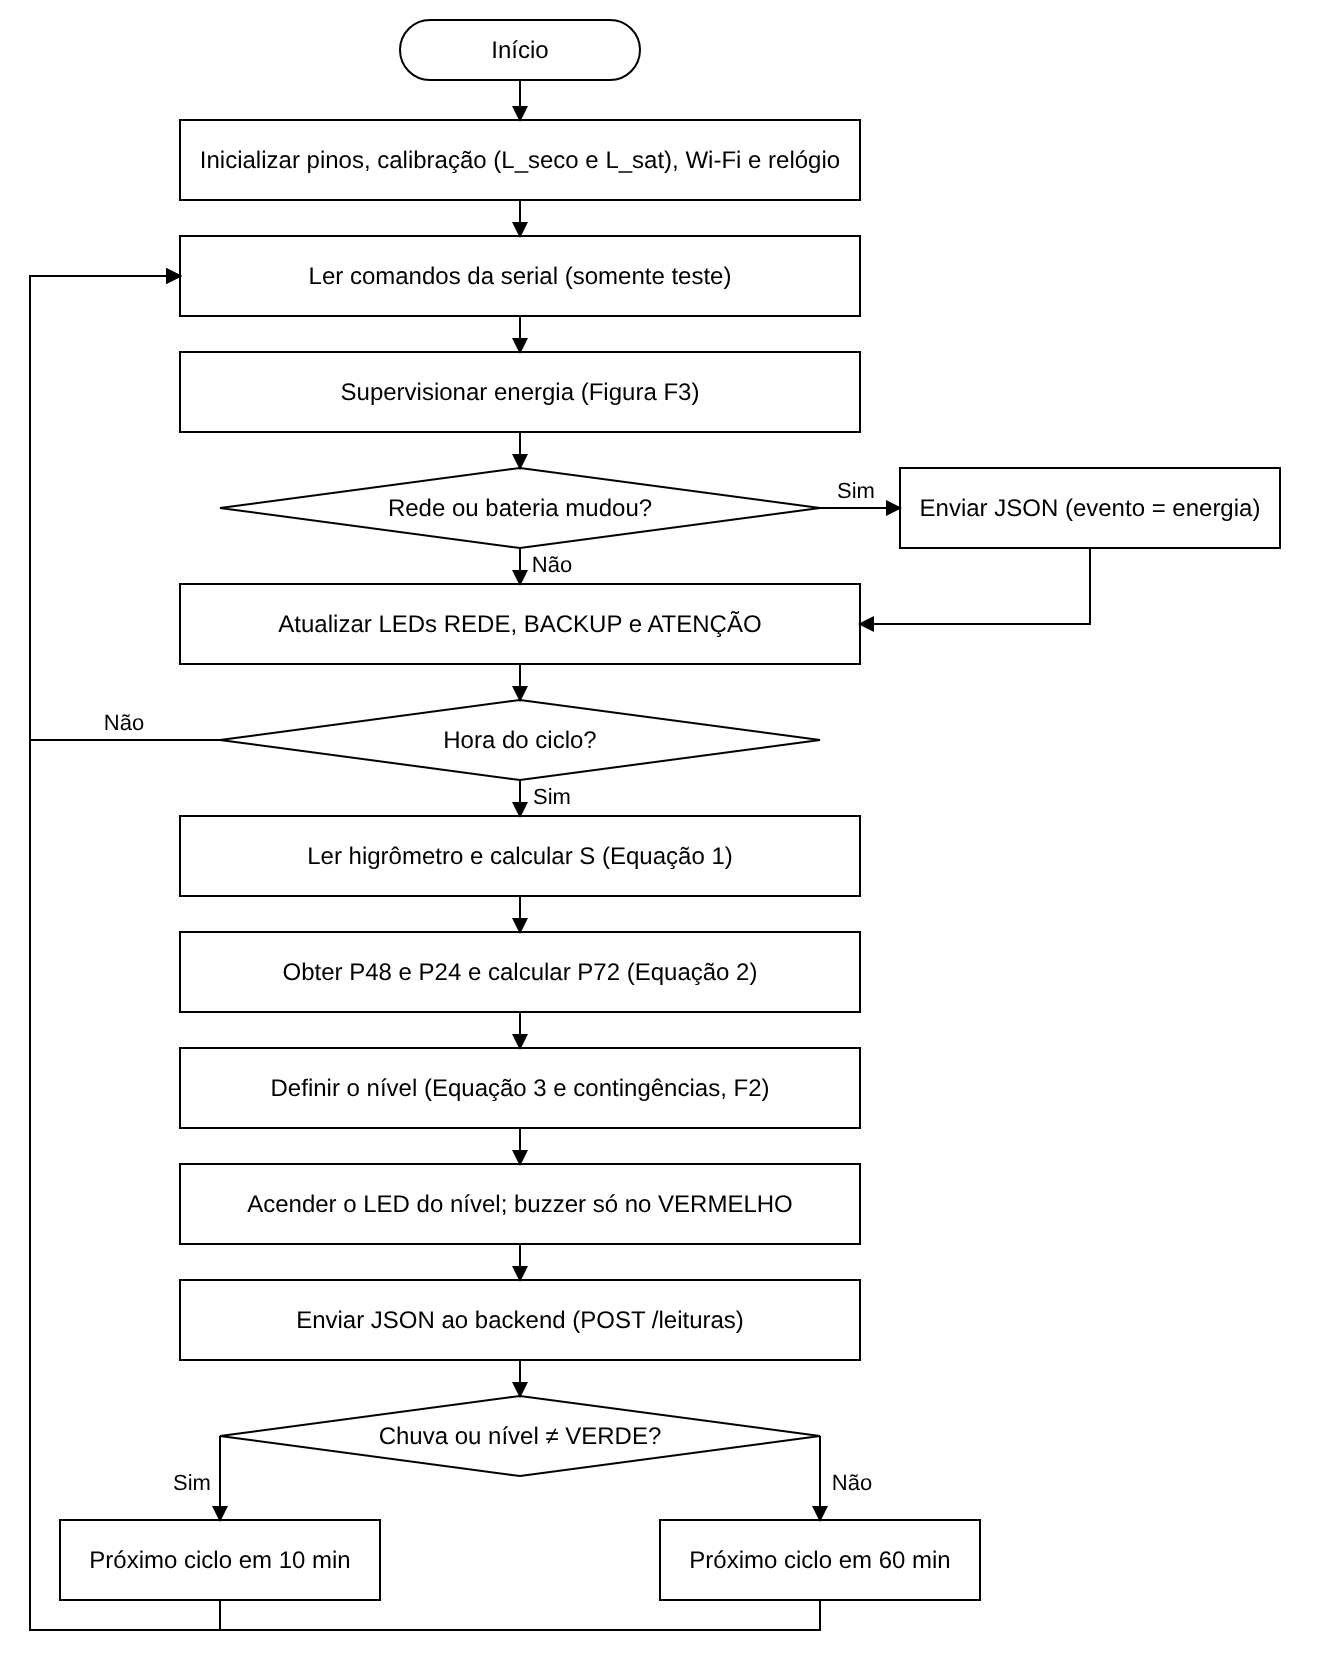
\includegraphics[width=\textwidth,height=0.85\textheight,keepaspectratio]{figures/image56_f1_fluxograma_geral.png}}
\caption{Fluxograma geral do dispositivo}
\label{fig:f1-geral}
\fonte{Elaborado pela autora, com utilização do draw.io (diagrams.net), 2026.}
\end{figure}

\paragraph*{Fluxograma do cálculo do nível}

A \autoref{fig:f2-nivel} detalha o cálculo do nível de alerta. A
leitura do higrômetro é convertida em $S$ pela \autoref{eq:saturacao},
e as parcelas de chuva são somadas pela \autoref{eq:p72}. Com os dois
dados disponíveis, o nível segue a \autoref{eq:nivel}, com os limiares
da \autoref{tab:limiares}.

Quando falta um dado, o fluxo segue as regras da
\autoref{subsec:contingencia}. Com dados de chuva incompletos, por
parcela não obtida ou por dia sem registro na estação, o nível usa o
mínimo garantido de $P_{72}$, desde que ele atinja $P_1$; abaixo disso,
os dados são tratados como indisponíveis e o fluxo segue pelo
conector B.

Sem o higrômetro, o nível depende só da chuva; sem os dados de chuva,
depende só de $S$; sem os dois, o nível é AMARELO, por precaução.

\begin{figure}[H]
\centering
\fbox{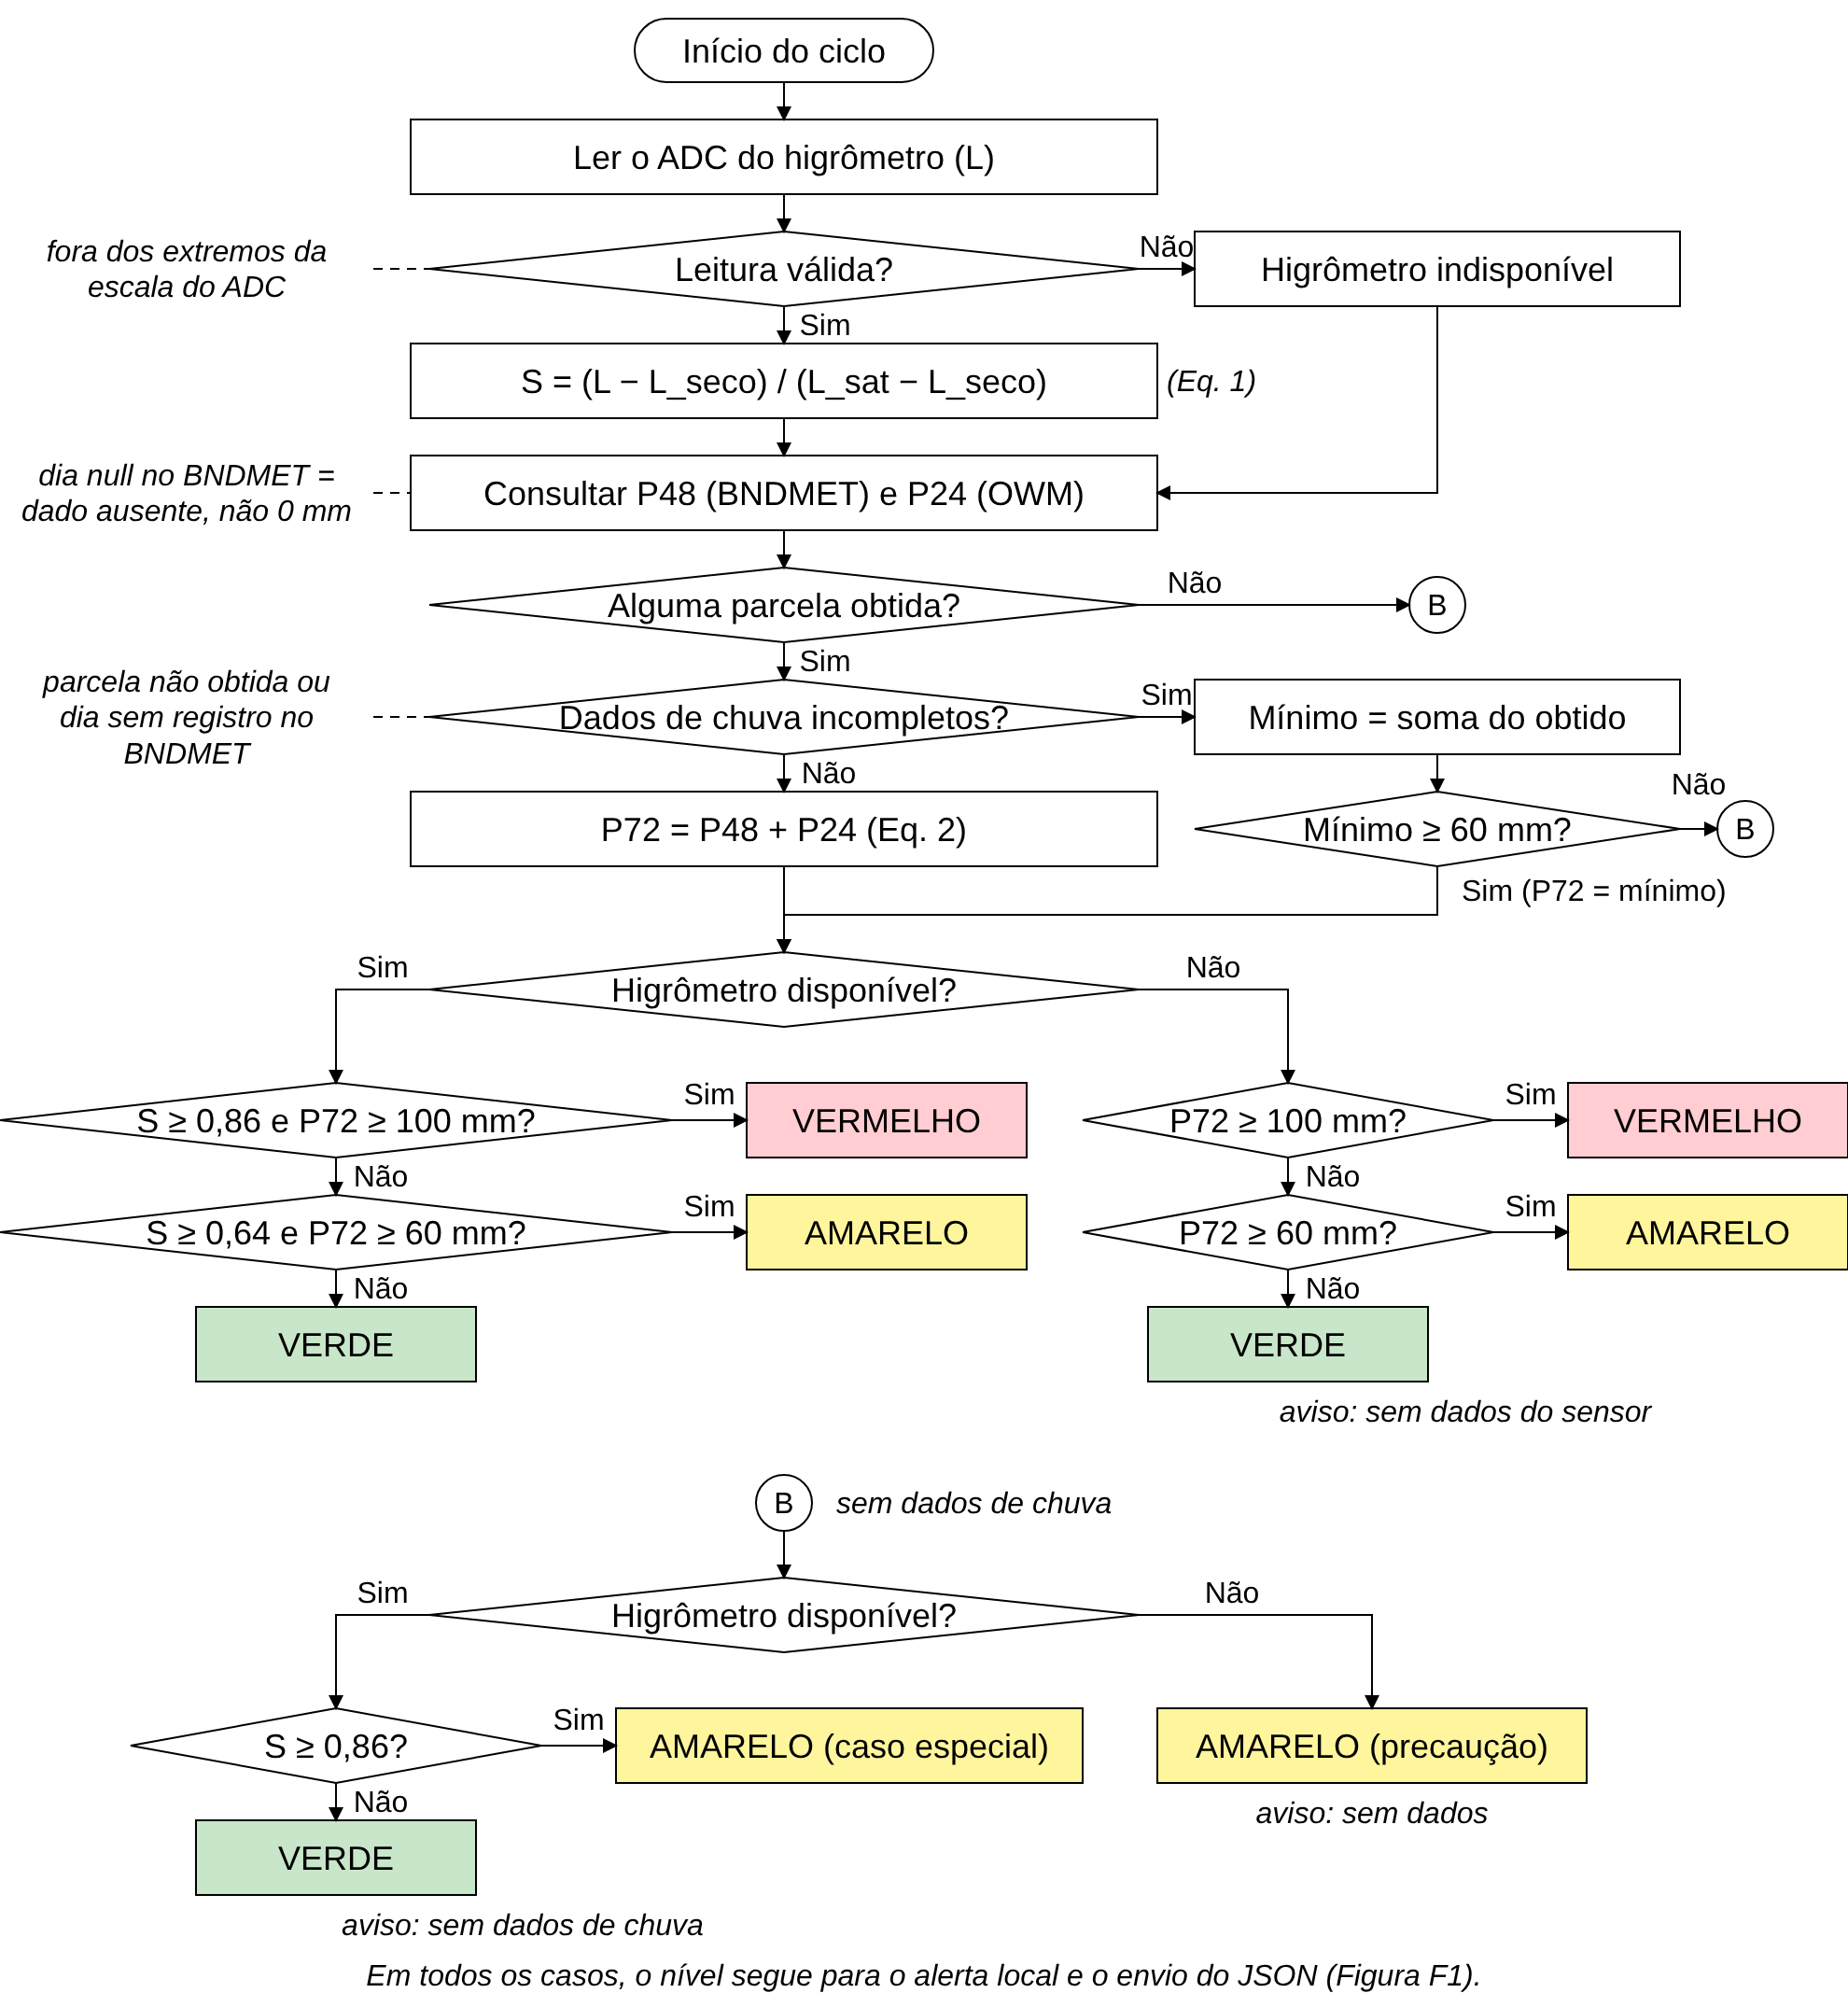
\includegraphics[width=\textwidth,height=0.85\textheight,keepaspectratio]{figures/image57_f2_calculo_nivel.png}}
\caption{Fluxograma do cálculo do nível de alerta}
\label{fig:f2-nivel}
\fonte{Elaborado pela autora, com utilização do draw.io (diagrams.net), 2026.}
\end{figure}

\paragraph*{Fluxograma da supervisão de energia}

A \autoref{fig:f3-energia} apresenta a supervisão de energia, presente
apenas na simulação. O dispositivo verifica a rede elétrica e a tensão
da bateria e classifica a bateria nos estados da
\autoref{tab:estados-energia}. A falha é indicada quando a rede está
presente e a bateria não completa a carga no tempo da
\autoref{eq:tempo-carga}.

A cada mudança da rede ou do estado da bateria, o dispositivo envia a
leitura ao \textit{backend}, que avisa os administradores por e-mail.
O cálculo do nível de alerta continua durante a operação na bateria.

\begin{figure}[H]
\centering
\fbox{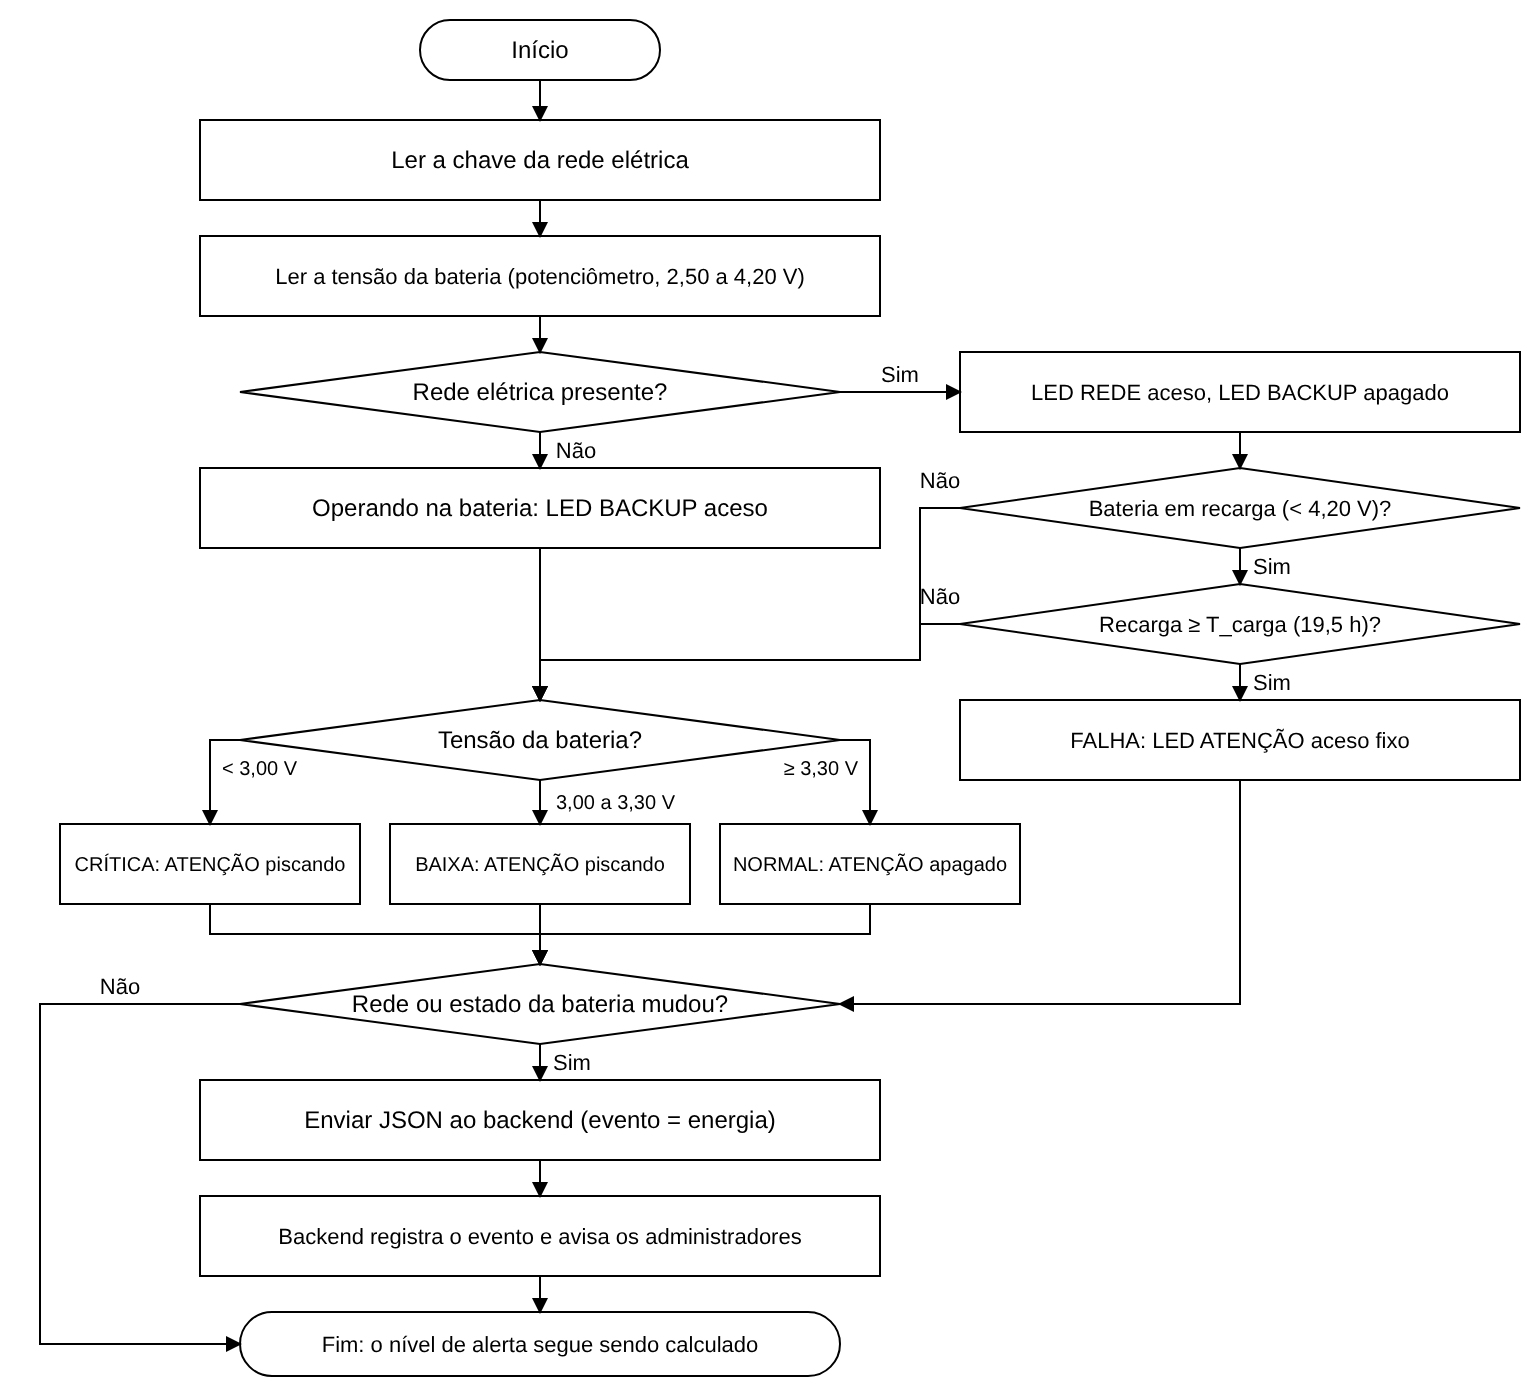
\includegraphics[width=\textwidth,height=0.85\textheight,keepaspectratio]{figures/image58_f3_energia.png}}
\caption{Fluxograma da supervisão de energia}
\label{fig:f3-energia}
\fonte{Elaborado pela autora, com utilização do draw.io (diagrams.net), 2026.}
\end{figure}

\paragraph*{Fluxograma do envio de e-mail de alerta}

A \autoref{fig:f4-email} apresenta o envio do e-mail de alerta pelo
administrador, após o \textit{login}. O administrador escolhe o nível,
e o sistema preenche a mensagem-modelo do nível
(\autoref{qua:mensagens-alerta}) com os dados da última leitura. O
texto pode ser editado antes do envio.

O envio exige pelo menos um morador cadastrado e a confirmação do
administrador. O sistema registra o envio, envia o e-mail aos
moradores ativos e informa ao administrador quantas mensagens foram
enviadas e quantas falharam.

\begin{figure}[H]
\centering
\fbox{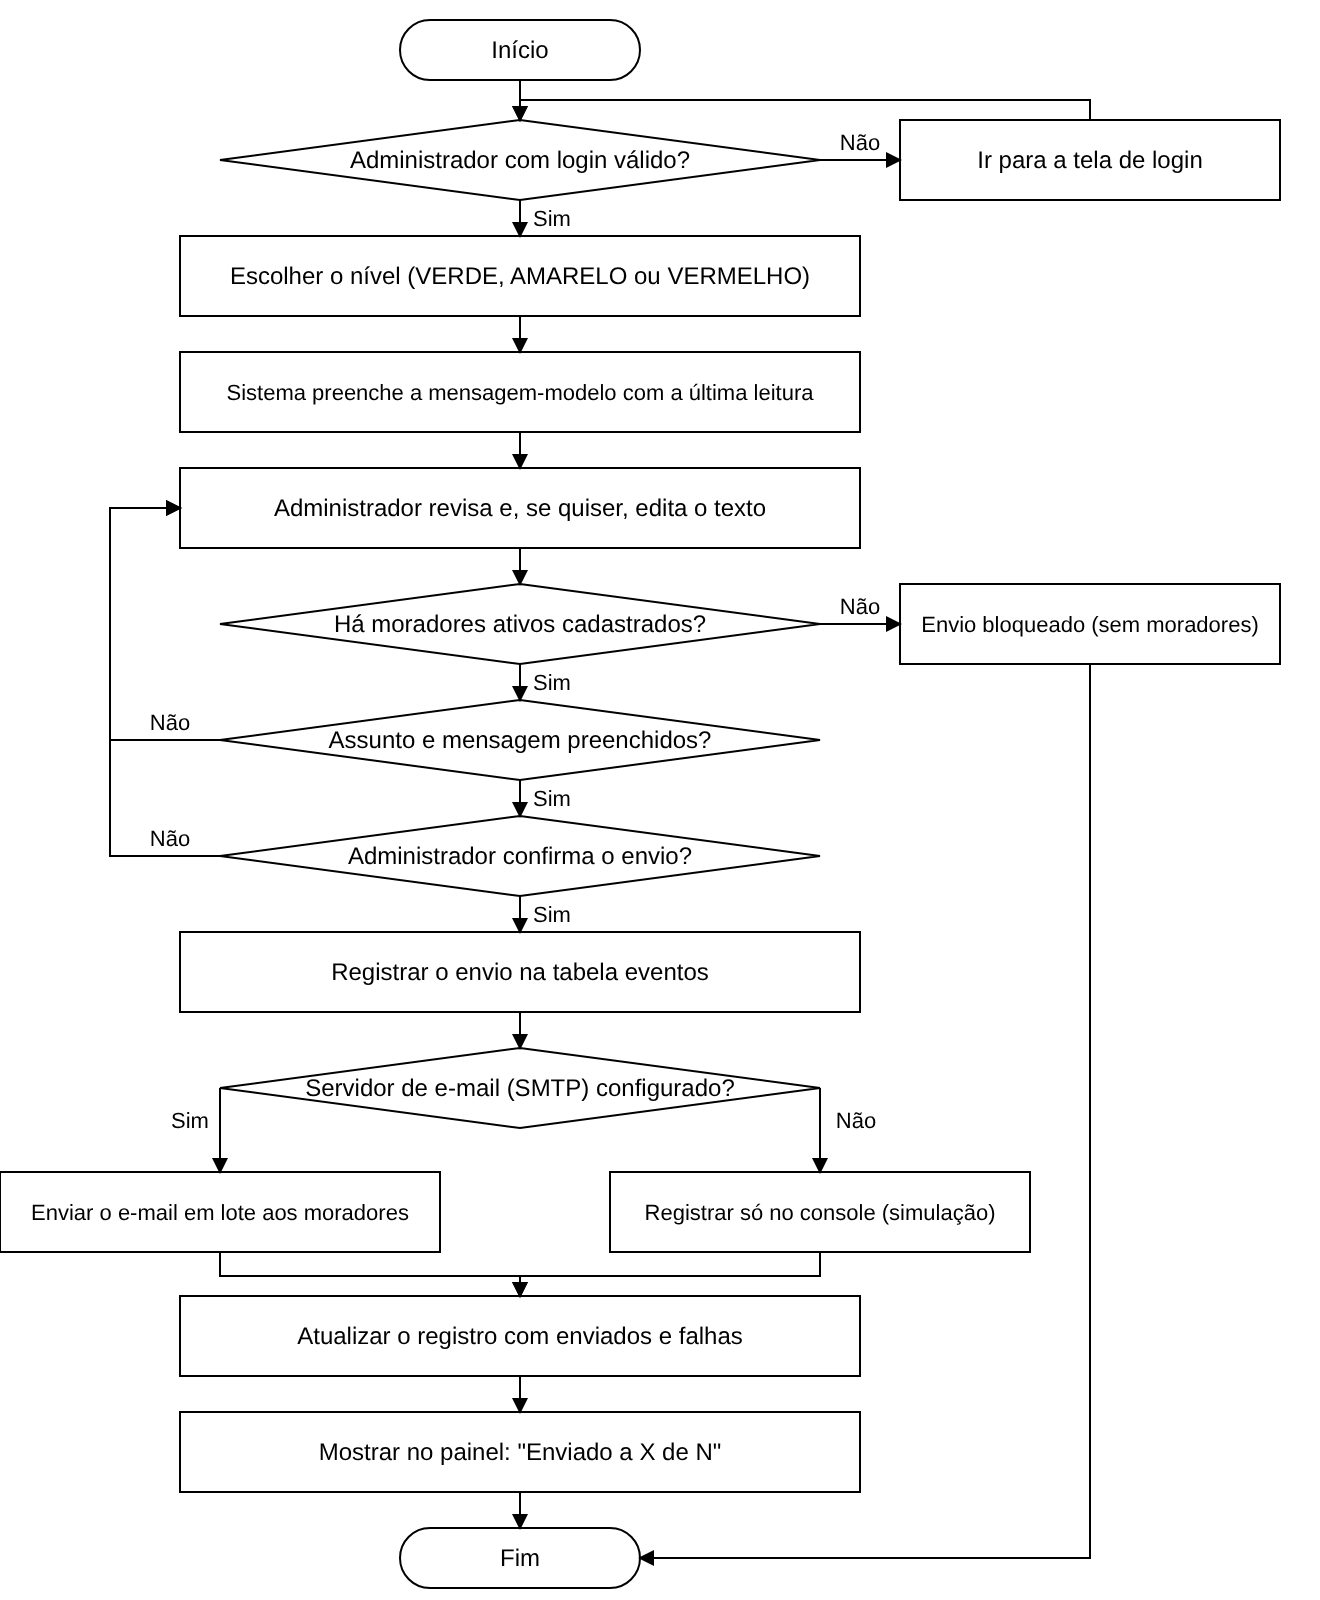
\includegraphics[width=\textwidth,height=0.85\textheight,keepaspectratio]{figures/image59_f4_envio_email.png}}
\caption{Fluxograma do envio do e-mail de alerta}
\label{fig:f4-email}
\fonte{Elaborado pela autora, com utilização do draw.io (diagrams.net), 2026.}
\end{figure}

\paragraph*{Diagrama de casos de uso}

O diagrama de casos de uso representa o que o sistema faz do ponto de
vista de quem interage com ele \cite{guedes2011uml}. A
\autoref{fig:casos-uso} apresenta cinco atores: o usuário básico
(morador), o administrador, o dispositivo e as APIs BNDMET e
OpenWeatherMap.

O dispositivo mede a saturação, consulta as APIs, calcula o nível,
aciona o alerta local e envia a leitura. O morador consulta a página
inicial e se cadastra para receber alertas. O administrador acompanha
o painel e envia o e-mail de alerta aos moradores, após o
\textit{login}. A seta parte do ator que inicia o caso de uso; a seta
com o rótulo ``destinatário'' indica o ator que apenas recebe o e-mail,
como o morador no envio do alerta.

\begin{figure}[H]
\centering
\fbox{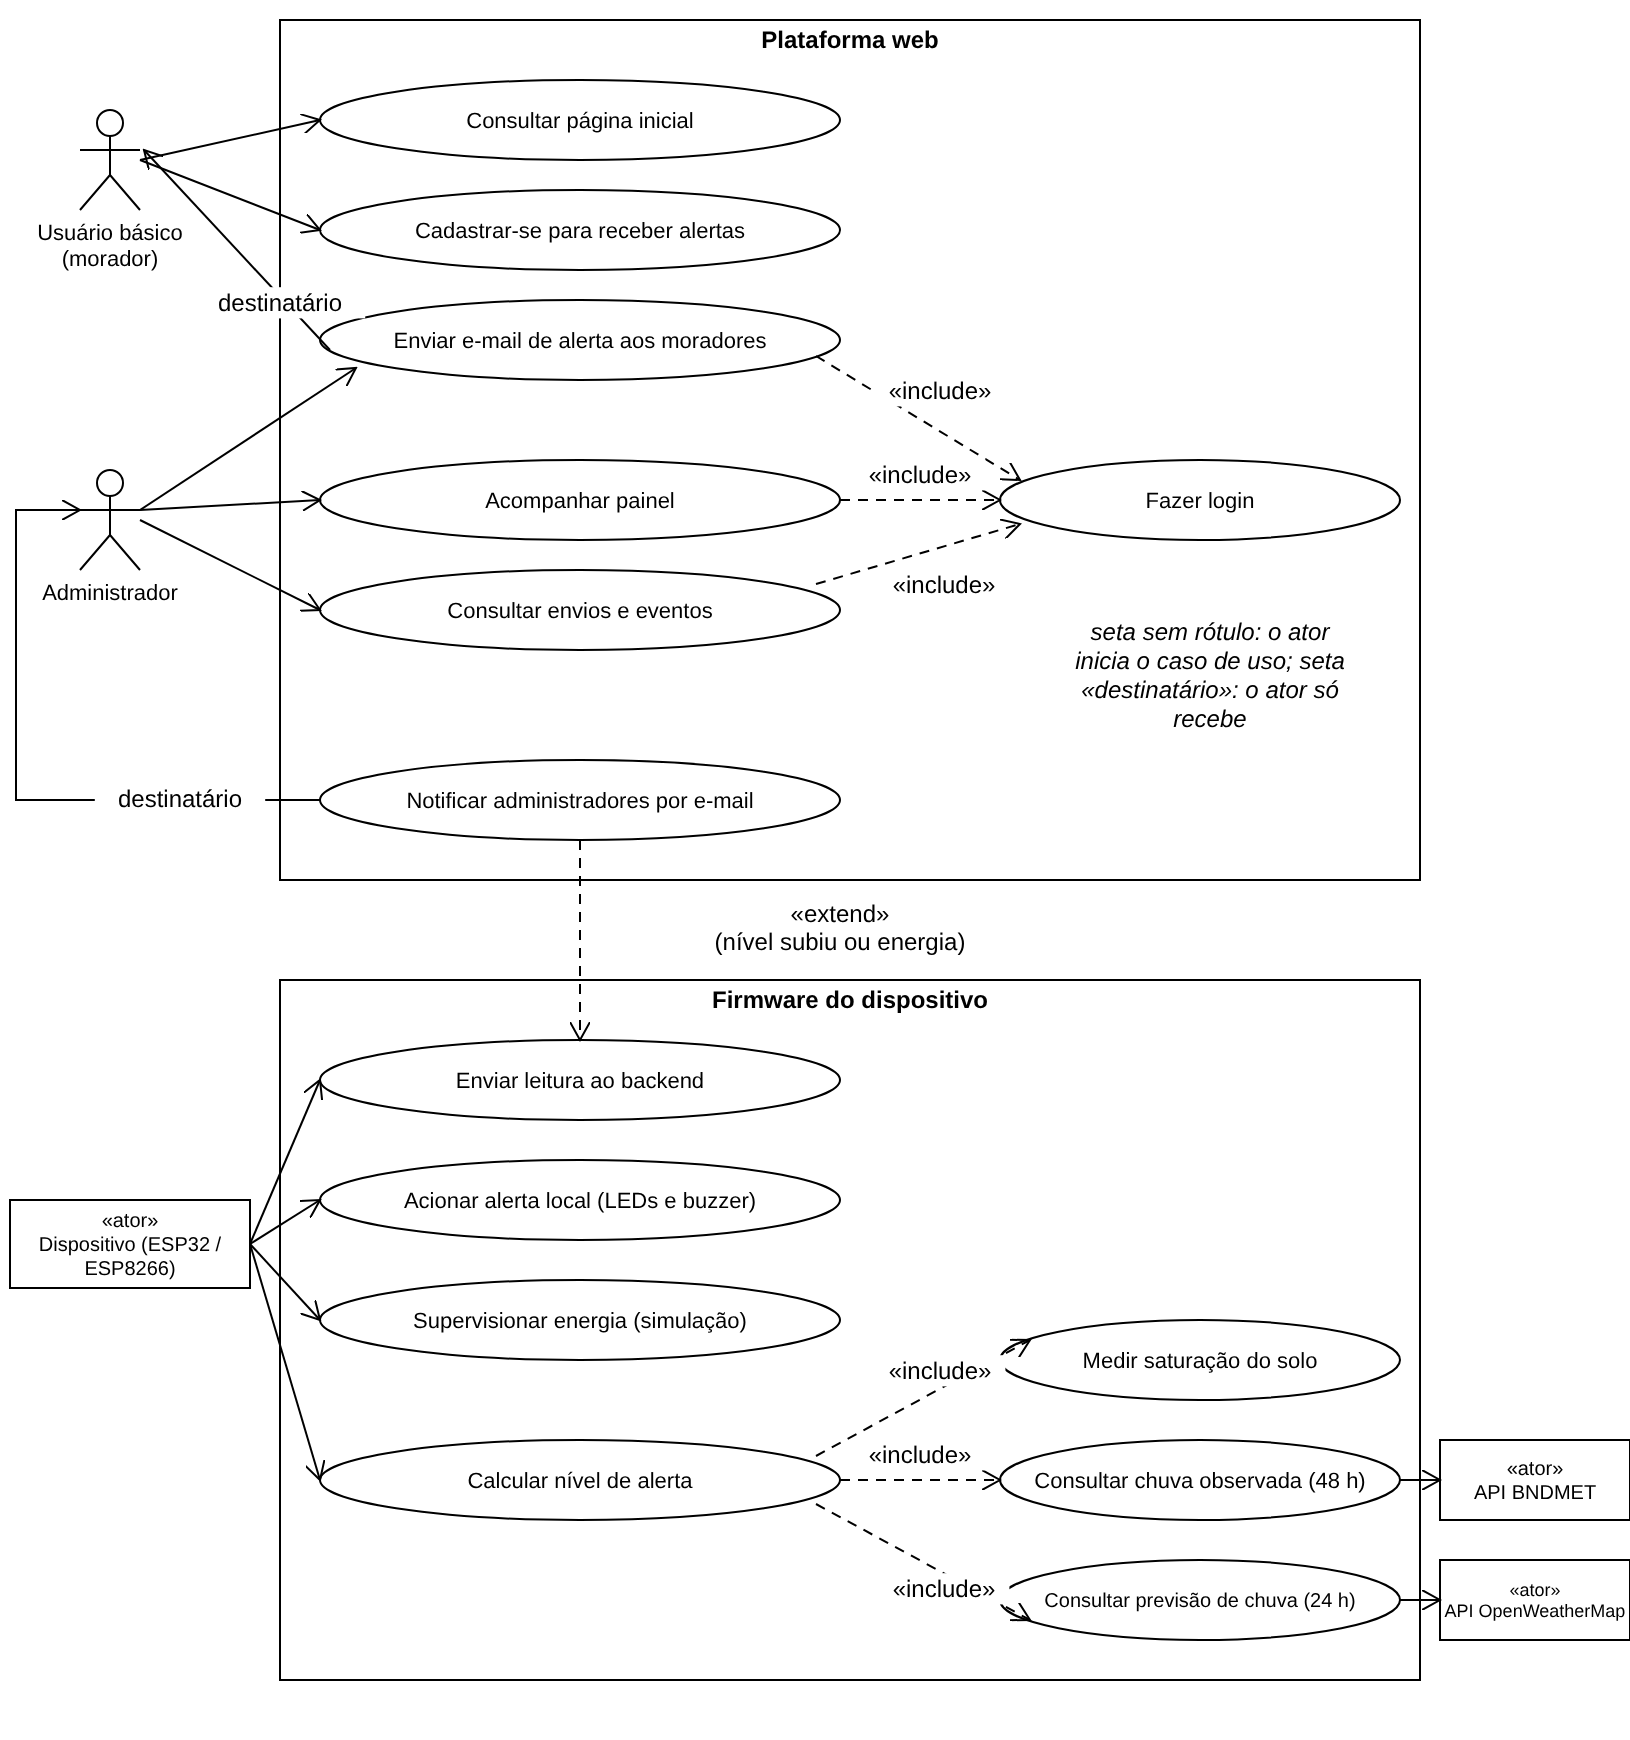
\includegraphics[width=\textwidth,height=0.85\textheight,keepaspectratio]{figures/image60_casos_de_uso.png}}
\caption{Diagrama de casos de uso}
\label{fig:casos-uso}
\fonte{Elaborado pela autora, com utilização do draw.io (diagrams.net), 2026.}
\end{figure}

\paragraph*{Diagrama de sequência}

O diagrama de sequência representa a ordem das mensagens trocadas
entre os componentes ao longo do tempo \cite{guedes2011uml}. Para
manter a legibilidade, ele foi dividido em duas partes, com numeração
contínua das mensagens.

A primeira parte (\autoref{fig:sequencia-1}) mostra o ciclo de leitura
do dispositivo. O dispositivo consulta as duas APIs, calcula o nível e
envia a leitura ao \textit{backend}, que a grava no banco de dados.

Se o nível subiu ou houve mudança de energia, o \textit{backend}
registra o evento e envia o e-mail aos administradores sem atrasar a
resposta ao dispositivo.

\begin{figure}[H]
\centering
\fbox{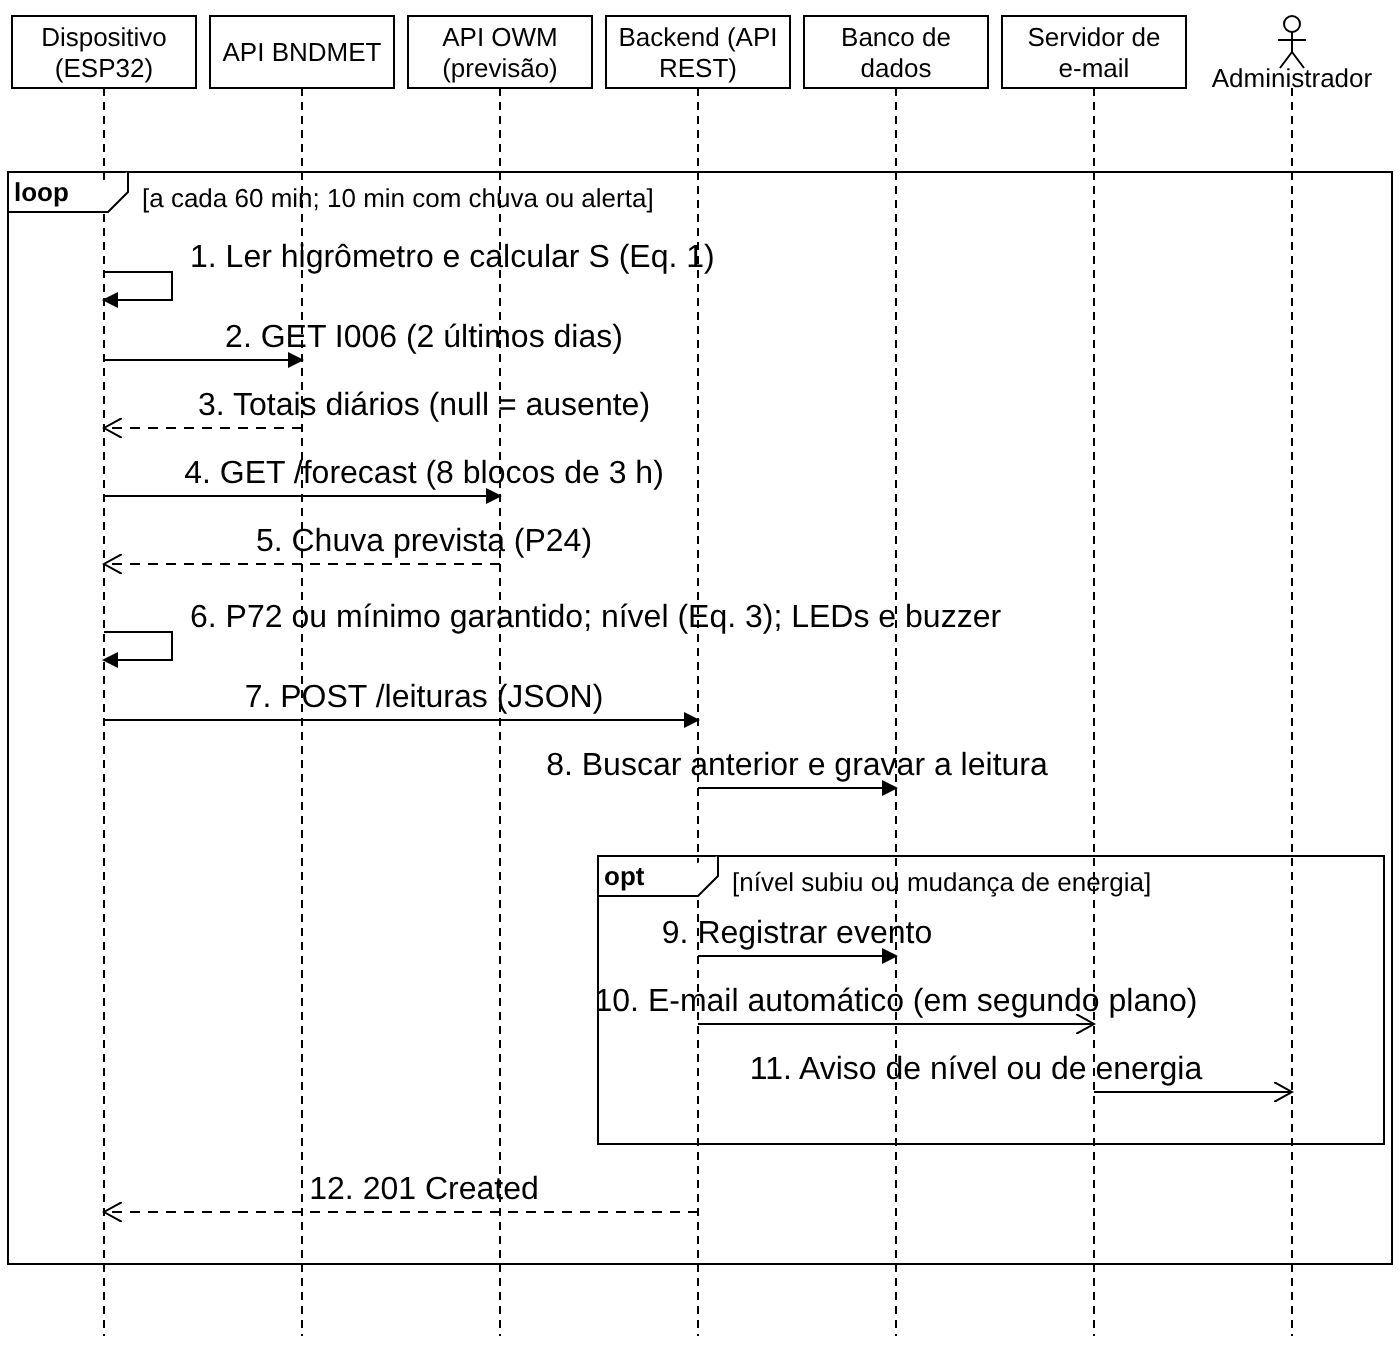
\includegraphics[width=\textwidth,height=0.85\textheight,keepaspectratio]{figures/image61_sequencia_1.png}}
\caption{Diagrama de sequência --- parte 1: ciclo de leitura do dispositivo}
\label{fig:sequencia-1}
\fonte{Elaborado pela autora, com utilização do draw.io (diagrams.net), 2026.}
\end{figure}

A segunda parte (\autoref{fig:sequencia-2}) mostra o uso do painel:
o \textit{login} do administrador, a atualização automática dos dados
e o envio do alerta aos moradores.

No envio do alerta, o administrador escolhe o nível e confirma a
mensagem. O \textit{backend} envia o e-mail aos moradores ativos e
registra o envio, com o número de mensagens enviadas e de falhas.

\begin{figure}[H]
\centering
\fbox{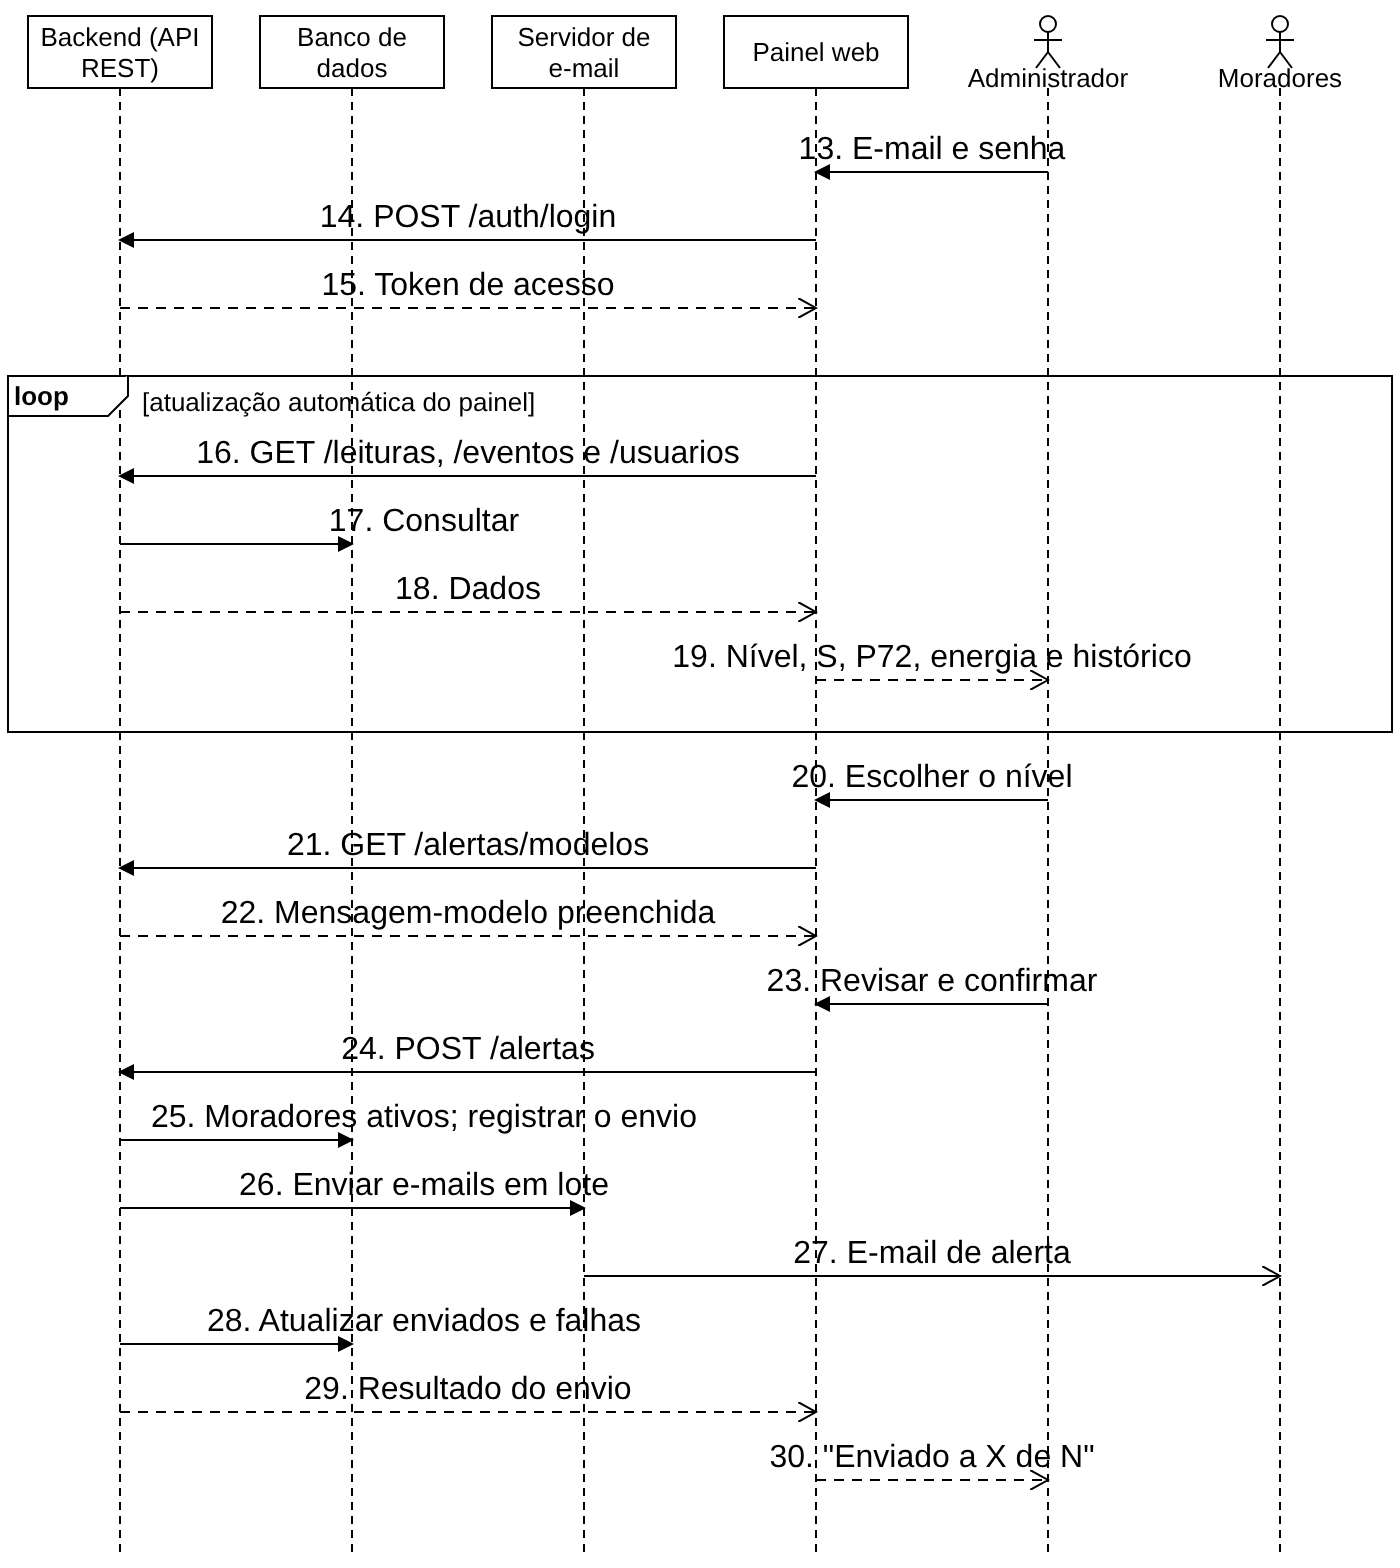
\includegraphics[width=\textwidth,height=0.85\textheight,keepaspectratio]{figures/image62_sequencia_2.png}}
\caption{Diagrama de sequência --- parte 2: painel e envio do alerta}
\label{fig:sequencia-2}
\fonte{Elaborado pela autora, com utilização do draw.io (diagrams.net), 2026.}
\end{figure}

O conteúdo das mensagens segue o Plano de Ação de Emergência previsto na Política
Nacional de Segurança de Barragens, que inclui o planejamento de rotas de fuga e
pontos de encontro, com a respectiva sinalização \cite{brasil2010pnsb,brasil2020lei14066}.
A mensagem do nível vermelho orienta o deslocamento, de forma análoga ao nível de
resposta vermelho do guia da \citeonline{ana2016manualpae}, em que o alerta à
população visa à evacuação. As cores do sistema não correspondem aos níveis de
emergência definidos pela \citeonline{anm2022resolucao95}.

\begin{quadro}[H]
\centering
\caption{Mensagens-modelo do e-mail de alerta}
\label{qua:mensagens-alerta}
\begin{tabular}{p{1.5cm}p{8.3cm}p{4.0cm}}
\hline
\textbf{Nível} & \textbf{Orientação ao morador} & \textbf{Base} \\
\hline
Verde & Não há necessidade de deslocamento. Conhecer a rota de fuga e o ponto de
encontro sinalizados e participar dos simulados. &
\citeonline{brasil2010pnsb}, art. 12, IV e XIII \\
Amarelo & Atenção. Confirmar a rota de fuga e o ponto de encontro; acompanhar novos
avisos e a Defesa Civil; seguir as orientações oficiais se a sirene tocar. &
\citeonline{ana2016manualpae}; \citeonline{brasil2010pnsb}, art. 12, XII e XIII \\
Vermelho & Deslocar-se imediatamente ao ponto de encontro pela rota de fuga
sinalizada e seguir as orientações da Defesa Civil. &
\citeonline{ana2016manualpae}; \citeonline{anm2022resolucao95}, art. 42 \\
\hline
\end{tabular}
\fonte{Elaborado pela autora com base em \citeonline{brasil2010pnsb},
\citeonline{ana2016manualpae} e \citeonline{anm2022resolucao95}.}
\end{quadro}

% =============================================================
\section{Protótipo de \textit{Hardware} Embarcado}
\label{sec:hardware}
% =============================================================

O protótipo físico é composto por quatro categorias de componentes: o
microcontrolador, o sensor de umidade, os indicadores visuais (LEDs) e o
indicador sonoro (\textit{buzzer}). Esses componentes são descritos nas
\autoref{subsec:esp8266} a \autoref{subsec:buzzer}.

A alimentação redundante, exigida de um sistema de alerta, é composta por
bateria, carregador e detecção da rede elétrica
(\autoref{subsec:bateria-carregador}). Ela foi dimensionada por cálculo
(\autoref{subsec:energia}) e representada na simulação
(\autoref{subsec:wokwi}), sem ser montada no protótipo físico.

% -------------------------------------------------------------
\subsection{ESP8266 NodeMCU V3}
\label{subsec:esp8266}
% -------------------------------------------------------------

O ESP8266 NodeMCU V3 é uma placa de desenvolvimento baseada no módulo
ESP-12E, equipada com processador de arquitetura 32 \textit{bits},
\textit{clock} de 80\,MHz, 4\,MB de memória \textit{flash} e 80\,KB
de RAM. Opera com tensão de 3,3\,V a nível lógico, admitindo
alimentação entre 5\,V e 9\,V via USB Tipo C. Possui 17 pinos GPIO,
conversor ADC de 10 \textit{bits} (pino A0), suporte a Wi-Fi 802.11
b/g/n em 2,4\,GHz com criptografia WPA/WPA2 e chip conversor USB-serial
CH340.

No protótipo, o ESP8266 lê o sensor de umidade, consulta as APIs
meteorológicas por HTTPS, calcula o nível de alerta, aciona os LEDs e o
\textit{buzzer} e envia os dados ao \textit{backend}
\cite{mercadolivre_esp8266, espressif_esp8266_spec2013}. A
\autoref{fig:esp8266} mostra a placa e a identificação dos seus pinos.

\begin{figure}[H]
    \centering
    \fbox{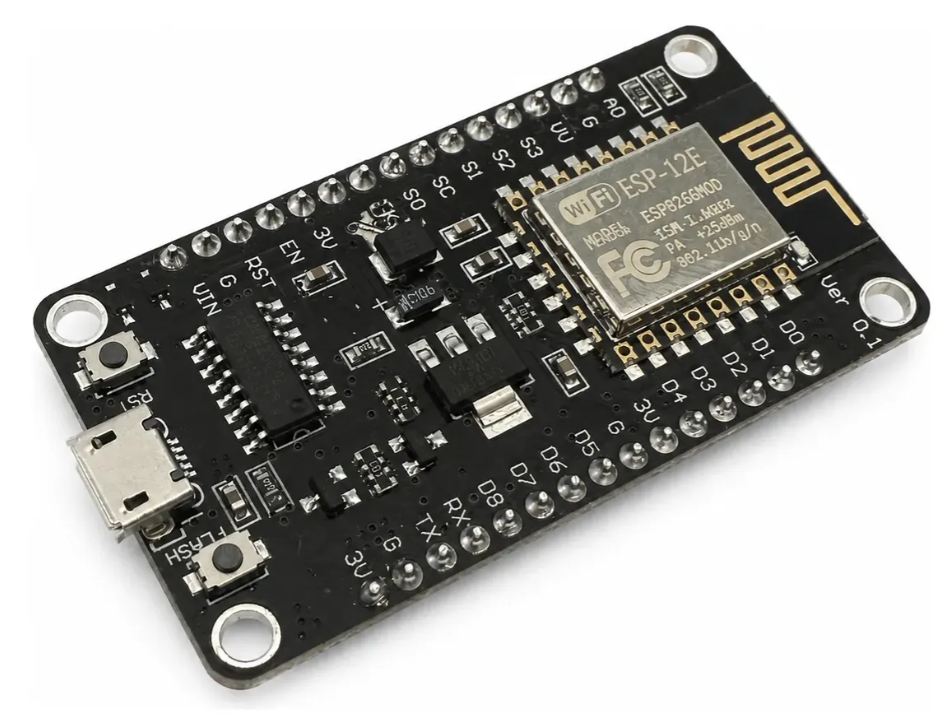
\includegraphics[width=0.7\textwidth]{figures/image63_esp8266_nodemcu.png}}
    \caption{Placa ESP8266 NodeMCU V3, com o módulo ESP-12E à esquerda, os pinos digitais na parte inferior, o pino analógico A0 no canto superior direito e o conector USB-C à esquerda}
    \label{fig:esp8266}
    \fonte{\citeonline{mercadolivre_esp8266}}
\end{figure}

O ESP8266EX possui um único conversor analógico-digital, de 10
\textit{bits}, no pino TOUT \cite[Seção~4.9]{espressif_esp8266ex}. Na
placa, esse conversor corresponde ao pino A0, ocupado pelo higrômetro.

% -------------------------------------------------------------
\subsection{Sensor Higrômetro Resistivo}
\label{subsec:higrometro}
% -------------------------------------------------------------

O módulo sensor de umidade de solo é composto por uma sonda resistiva
FC-28 e por uma placa com o comparador LM393, com saída analógica (A0) e
digital (D0) e tensão de operação entre 3,3\,V e 5\,V
\cite{eletrogate_higrometro,dfrobot_sen0114}. A placa mede
3$\times$1,5\,cm, e a sonda, 6$\times$2\,cm \cite{eletrogate_higrometro}.
A \autoref{fig:higrometro} mostra a sonda, que é inserida no solo, e a
placa com o comparador, ligadas por um cabo.

\begin{figure}[H]
    \centering
    \fbox{\includegraphics[width=0.5\textwidth]{figures/image50_higrometro.png}}
    \caption{Módulo sensor de umidade de solo: sonda FC-28, à direita, e placa com o comparador LM393, à esquerda}
    \label{fig:higrometro}
    \fonte{\citeonline{eletrogate_higrometro}}
\end{figure}

No protótipo, apenas a saída analógica é utilizada, ligada ao pino A0 do
ESP8266. A leitura do conversor é transformada na saturação relativa $S$,
de 0 a 1, pela \autoref{eq:saturacao}.

As leituras com o solo seco e com o solo saturado, usadas nessa equação,
são obtidas por calibração e gravadas na memória EEPROM do
microcontrolador. Assim, a calibração é mantida após uma reinicialização.

A leitura do sensor e o envio dos dados ao \textit{backend} seguem os
intervalos de registro dos pluviômetros do Cemaden: 60 minutos sem chuva e
10 minutos com chuva \cite[p.~2]{freitas2021analise}. A regra adotada e
seu efeito no consumo são descritos na \autoref{subsec:energia}.

% -------------------------------------------------------------
\subsection{LEDs Indicadores}
\label{subsec:leds}
% -------------------------------------------------------------

Foram utilizados três LEDs difusos de 5\,mm para sinalizar o nível de
alerta, ligados aos pinos D1 (azul), D2 (amarelo) e D3 (vermelho). Apenas
o LED do nível atual permanece aceso (\autoref{fig:leds}).

\begin{figure}[H]
    \centering
    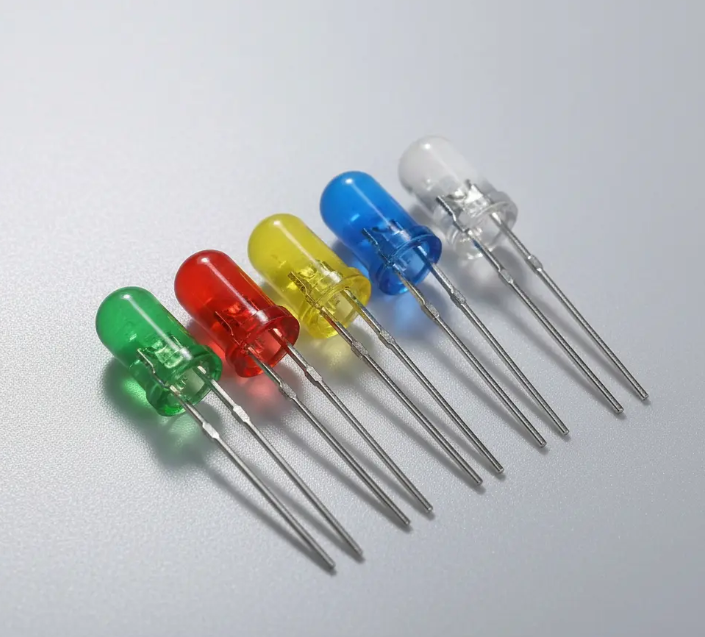
\includegraphics[width=0.55\textwidth]{figures/image64_leds.png}
    \caption{LEDs indicadores de 5\,mm e o nível de alerta sinalizado por cada um}
    \label{fig:leds}
    \fonte{\citeonline{mercadolivre_leds}}
\end{figure}

No protótipo físico, o nível VERDE é indicado pelo LED azul, componente
disponível na montagem. A cor não altera a lógica de alerta: o
\textit{firmware} aciona o pino D1 no nível VERDE. Na simulação, esse
nível é indicado por um LED verde (\autoref{subsec:wokwi}).

O LED azul opera entre 3,0 e 3,3\,V, com corrente máxima de 20\,mA e
ângulo de abertura de 60° \cite{usinainfo_led_azul}. O amarelo opera
entre 2,0 e 2,2\,V, com 20\,mA, e o vermelho, a 1,8\,V, com 15\,mA;
ambos têm ângulo de abertura de 120°
\cite{usinainfo_led_amarelo,usinainfo_led_vermelho}.

Os LEDs foram ligados diretamente aos pinos, sem resistor em série. Por
isso, a corrente de cada LED foi considerada igual ao limite de corrente do
pino, de 12\,mA \cite[Tabela~5-1]{espressif_esp8266ex}, conforme a
\autoref{tab:consumo}.

% -------------------------------------------------------------
\subsection{\textit{Buzzer} Ativo TMB-12A03}
\label{subsec:buzzer}
% -------------------------------------------------------------

O \textit{buzzer} ativo TMB-12A03 está ligado ao pino D4 do ESP8266. Por
ser ativo, possui oscilador interno e emite som quando recebe nível
lógico alto, sem controle de frequência por \textit{software}
\cite{quickteck_tmb12a03}.

O \textit{buzzer} é acionado apenas no nível VERMELHO. Os níveis VERDE e
AMARELO são indicados somente pelos LEDs.

Segundo o fabricante, o TMB-12A03 tem tensão nominal de 3\,V (faixa de
2,5 a 4\,V), corrente de até 35\,mA, nível sonoro mínimo de 82\,dB a
10\,cm, frequência de ressonância de 2300\,$\pm$\,500\,Hz e diâmetro de
12\,mm \cite{quickteck_tmb12a03}. A \autoref{fig:buzzer} mostra o
componente, com o terminal positivo ligado ao pino D4.

\begin{figure}[H]
    \centering
    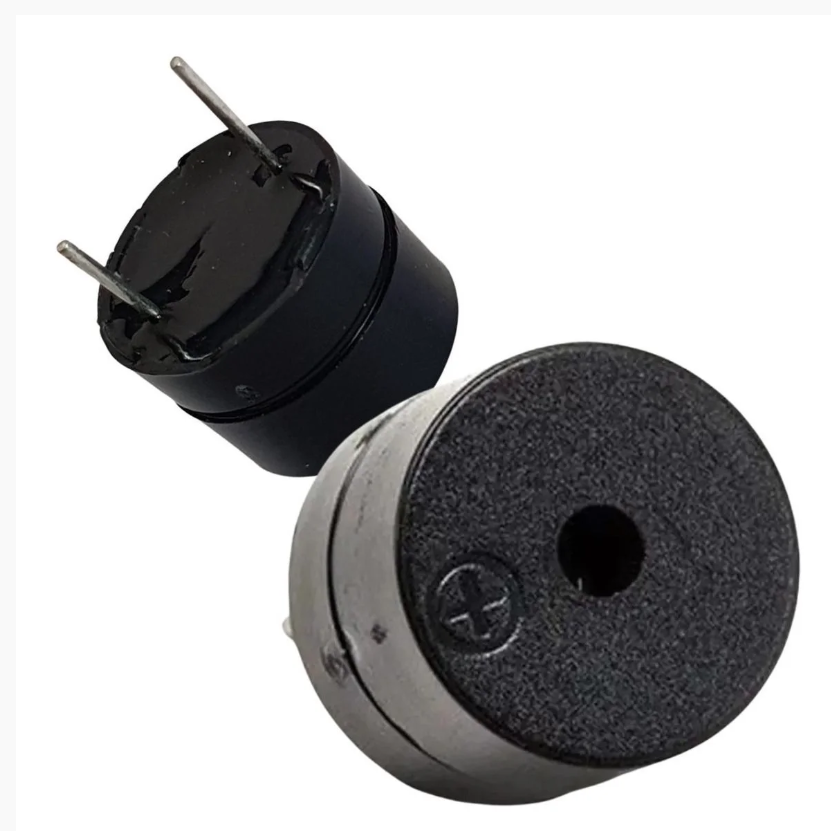
\includegraphics[width=0.6\textwidth]{figures/image65_buzzer_tmb12a03.png}
    \caption{\textit{Buzzer} ativo TMB-12A03: vista superior e vista lateral, com as dimensões e os terminais}
    \label{fig:buzzer}
    \fonte{\citeonline{smartcomponentes_buzzer}.}
\end{figure}

% -------------------------------------------------------------
\subsection{Bateria, Carregador e Detecção da Rede}
\label{subsec:bateria-carregador}
% -------------------------------------------------------------

Os componentes desta subseção foram especificados para a alimentação
redundante e não foram montados no protótipo físico. A quantidade de
células resulta do cálculo da \autoref{subsec:energia}.

A bateria é formada por três células de íon-lítio Panasonic NCR18650B
ligadas em paralelo, cada uma em um suporte individual. Cada célula tem
capacidade nominal mínima de 3200\,mAh e tensão nominal de 3,6\,V
\cite{panasonic_ncr18650b}.

Foi especificada a versão da célula com circuito de proteção, que a
desliga em 2,50\,V \cite{bto_ncr18650_pcm}. Essa proteção é necessária
porque o módulo de alimentação não protege a célula contra descarga
profunda.

O módulo de referência para carregar a bateria e alimentar a placa é o
PowerBoost 1000C. Ele combina um carregador com compartilhamento de carga,
que alimenta o circuito e carrega a bateria ao mesmo tempo, e um conversor
elevador com saída de 5,2\,V \cite{adafruit_powerboost1000c,microchip_mcp73871}.

A presença da rede elétrica pode ser obtida do próprio carregador. A
saída PG (\textit{power-good}) do MCP73871 fica em nível baixo sempre que
uma fonte externa, e não a bateria, alimenta o circuito
\cite[Seção~5.2.4]{microchip_mcp73871}.

A tensão da bateria exigiria uma entrada analógica. No ESP8266, a única
entrada desse tipo já é usada pelo higrômetro (\autoref{subsec:esp8266}).
Por isso, a supervisão de energia foi implementada apenas na simulação,
em que uma chave representa a saída de rede presente e um potenciômetro
representa a tensão da bateria (\autoref{subsec:wokwi}).

% -------------------------------------------------------------
\subsection{Diagrama de Circuito e Conexões}
\label{subsec:circuito}
% -------------------------------------------------------------

A \autoref{fig:componentes_ligados} apresenta o diagrama de montagem do
protótipo, elaborado no \textit{software} Fritzing, e a
\autoref{fig:esquematico}, o esquemático elétrico correspondente, com os
pinos e as ligações entre os componentes.

\begin{figure}[H]
\centering
\fbox{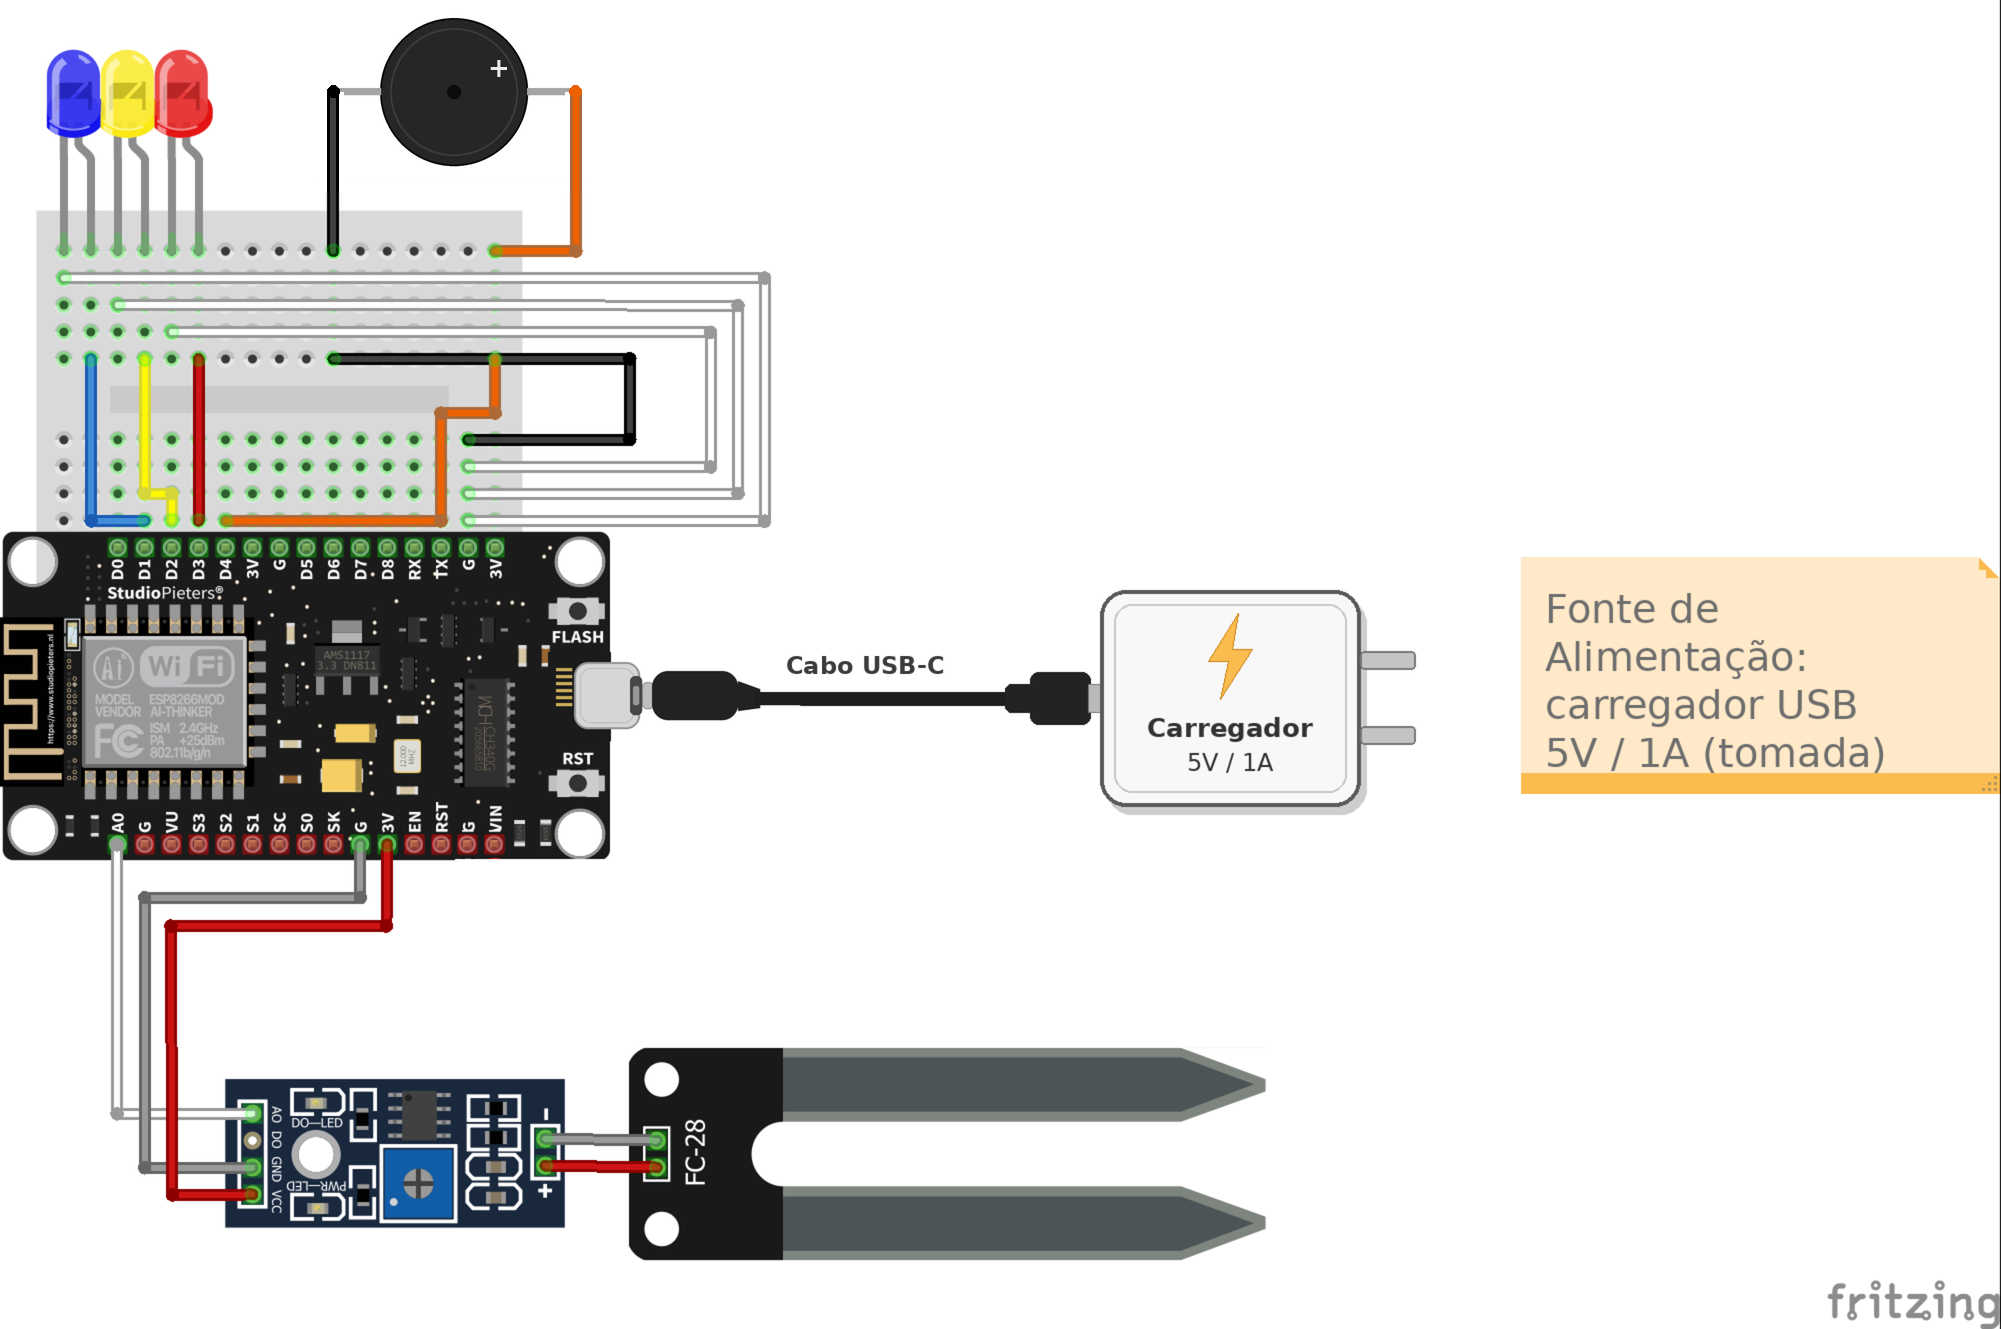
\includegraphics[width=\textwidth]
    {figures/image51_componentes_ligados_versao_3_bb.png}}
\caption{Diagrama de montagem do protótipo embarcado}
\label{fig:componentes_ligados}
\fonte{Autora, 2026.}
\end{figure}

\begin{figure}[H]
\centering
\fbox{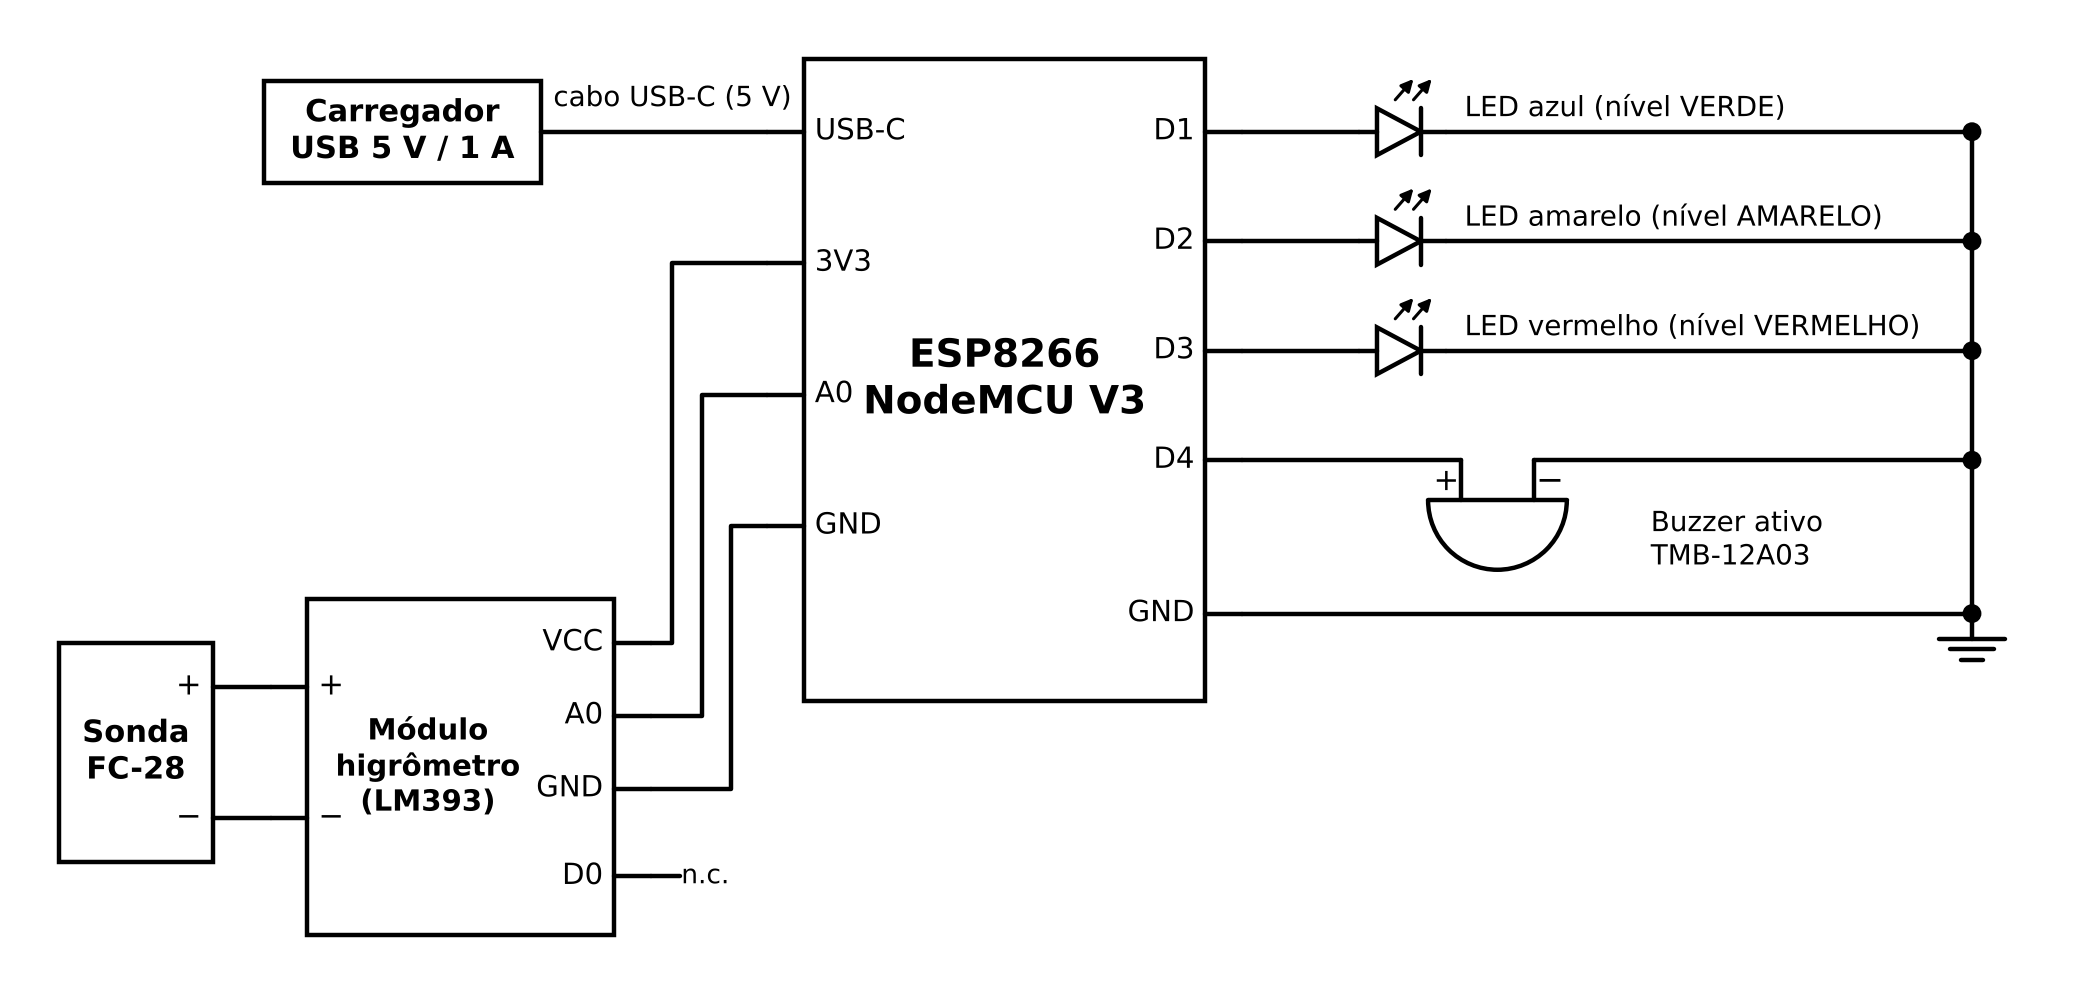
\includegraphics[width=\textwidth]
        {figures/image52_esquematico_versao_3.png}}
    \caption{Esquemático elétrico do protótipo embarcado}
    \label{fig:esquematico}
    \fonte{Elaborado pela autora, com utilização da biblioteca Matplotlib (Python), 2026.}
\end{figure}

Na montagem, o LED azul indica o nível VERDE (\autoref{subsec:leds}), e a
placa é alimentada por um carregador de 5\,V pela porta USB-C. A
alimentação redundante não aparece na figura, pois não foi montada
(\autoref{subsec:bateria-carregador}).

A transmissão dos dados coletados por este circuito ao restante do
sistema é descrita na \autoref{subsec:arquitetura}: o \textit{firmware}
calcula o nível de alerta, monta um objeto JSON com o nível, os valores
de $S$, $P_{48}$, $P_{24}$ e $P_{72}$ (ou o mínimo garantido de
$P_{72}$, quando os dados de chuva estão incompletos) e os avisos de
dado incompleto ou indisponível,
e o envia ao \textit{backend} pela rota \texttt{POST /leituras}
(\autoref{fig:sequencia-1}).

% -------------------------------------------------------------
\subsection{Especificações Técnicas e Custos}
\label{subsec:specs-custos}
% -------------------------------------------------------------

A Tabela~\ref{tab:specs} consolida as principais especificações
técnicas dos componentes utilizados.

\begin{table}[H]
\centering
\caption{Especificações técnicas dos componentes do protótipo e da alimentação redundante}
\label{tab:specs}
\small
\begin{tabular}{p{5.5cm}p{2.9cm}p{3.6cm}p{3.0cm}}
\hline
\textbf{Componente} & \textbf{Tensão (V)} & \textbf{Corrente} & \textbf{Interface} \\
\hline
ESP8266 NodeMCU V3 & 3,3 (lógico) & 80\,mA (média); até 215\,mA (TX contínuo) & Wi-Fi / GPIO / ADC \\
Módulo higrômetro (comparador LM393) & 3,3 ou 5 & 35\,mA (módulo); LM393: até 1,0\,mA & Analógica (A0) \\
LED azul 5\,mm (nível VERDE) & 3,0--3,3 & 20\,mA & GPIO digital \\
LED amarelo 5\,mm & 2,0--2,2 & 20\,mA & GPIO digital \\
LED vermelho 5\,mm & 1,8 & 15\,mA & GPIO digital \\
\textit{Buzzer} ativo TMB-12A03 & 3 (faixa 2,5--4) & até 35\,mA & GPIO digital \\
\hline
\multicolumn{4}{l}{\textit{Alimentação redundante (especificada; não montada no protótipo físico)}} \\
\hline
Célula Li-ion NCR18650B (3 em paralelo) & 3,6 (nominal); 4,20 (carga); 2,50 (corte) & carga padrão: 1625\,mA por célula & -- \\
Módulo carregador e elevador (referência PowerBoost 1000C) & 5,2 (saída) & carga: até 1000\,mA & USB \\
\hline
\end{tabular}
\fonte{Elaborado pela autora com base em \citeonline{espressif_esp8266ex,espressif_esp8266_spec2013,aithinker_esp12e,dfrobot_sen0114,ti_lm393,usinainfo_led_azul,usinainfo_led_amarelo,usinainfo_led_vermelho,quickteck_tmb12a03,panasonic_ncr18650b,adafruit_powerboost1000c}.}
\end{table}

O custo dos componentes do protótipo físico foi de R\$\,70,30. A
\autoref{tab:custos} apresenta também os itens da alimentação redundante,
especificados na \autoref{subsec:energia}, que não foram montados. Com
eles, o custo total passa a R\$\,602,70.

\begin{table}[H]
\centering
\caption{Componentes e custos do protótipo embarcado}
\label{tab:custos}
\begin{tabular}{p{11.0cm}cc}
\hline
\textbf{Componente} & \textbf{Qtd.} & \textbf{Custo (R\$)} \\
\hline
ESP8266 NodeMCU V3 & 1 & 59,90 \\
Higrômetro resistivo LM393 & 1 & 7,50 \\
\textit{Buzzer} ativo 12\,mm & 1 & 2,30 \\
LEDs indicadores (conjunto) & 1 & 0,60 \\
\hline
\textbf{Subtotal do protótipo físico} & & \textbf{70,30} \\
\hline
Célula Li-ion Panasonic NCR18650B com proteção$^{\mathrm{a}}$ & 3 & 312,64 \\
Suporte para uma célula 18650 (ligados em paralelo) & 3 & 14,19 \\
Módulo carregador e elevador PowerBoost 1000C (MCP73871 + TPS61090) & 1 & 205,57 \\
\hline
\textbf{Subtotal da alimentação redundante} & & \textbf{532,40} \\
\hline
\textbf{Total} & & \textbf{602,70} \\
\hline
\end{tabular}
\fonte{Autora, 2026, com preços consultados em 4 out. 2026, sem frete
\cite{taklite_ncr18650b_pcb,usinainfo_suporte_18650,amazon_powerboost1000c}.}
\nota{$^{\mathrm{a}}$Preço unitário de US\$\,19,95, convertido pela taxa
PTAX de venda de 2 out. 2026, de R\$\,5,2238 \cite{piranot2026ptax}, sem
impostos de importação.}
\end{table}

O protótipo físico é alimentado por fonte externa de 5\,V, pela porta
USB-C. A alimentação redundante por bateria, exigida de um sistema de
alerta, foi dimensionada por cálculo e demonstrada na simulação, conforme
a \autoref{subsec:energia}.

% -------------------------------------------------------------
\subsection{Alimentação Redundante e Supervisão de Energia}
\label{subsec:energia}
% -------------------------------------------------------------

Esta subseção especifica a alimentação de reserva do sistema e a
dimensiona por cálculo, a partir dos \textit{datasheets} dos componentes
do protótipo. A bateria não foi montada no protótipo físico. Sua lógica de
supervisão foi representada na simulação (\autoref{subsec:wokwi}), na qual
o ESP32 e os componentes virtuais não reproduzem o consumo real.

\paragraph*{Necessidade da alimentação redundante}

Um sistema de alerta precisa continuar operando quando a rede elétrica
falha. Ventos fortes e tempestades podem derrubar galhos e árvores sobre
as redes elétricas e causar interrupções de energia
\cite[p.~10]{aneel2024nt90}.

São justamente os períodos de chuva intensa que fornecem o gatilho do
modelo de alerta (\autoref{sec:modelo-risco}). Sem reserva de energia, o
dispositivo deixaria de medir, de calcular o nível e de alertar quando o
risco é maior.

A Política Nacional de Segurança de Barragens também prevê, no plano de
emergência, um sistema sonoro ou outra solução tecnológica para situações
de alerta \cite{brasil2010pnsb,brasil2020lei14066}.

\paragraph*{Requisito de autonomia}

Não foi encontrada norma de autonomia específica para dispositivos de
monitoramento de barragens. Adotou-se, por analogia, o requisito das
normas de sistemas de alarme, que tratam de equipamentos que também
precisam sinalizar durante a falta de energia.

A IT~14 do Corpo de Bombeiros de Minas Gerais, estado da área de estudo,
exige autonomia mínima de 24 horas em regime de supervisão e de 15
minutos em regime de alarme \cite[item~5.3]{cbmmg2017it14}. A NT~19/2022
de Goiás traz o mesmo requisito \cite[item~5.3]{cbmgo2022nt19}.

A NFPA~72 exige 24 horas de supervisão seguidas de 5 minutos de alarme,
ou 15 minutos em sistemas com voz
\cite{hammerberg2021calculation,reiswig2023nfpa72}. Adotou-se o requisito
mais exigente: 24 horas de supervisão e 15 minutos de alarme.

\paragraph*{Consumo por componente}

A \autoref{tab:consumo} apresenta a corrente de cada componente na
entrada de 5\,V da placa, em dois regimes. Em supervisão, o nível é VERDE
ou AMARELO, com um LED aceso. Em alarme, o nível é VERMELHO, com o LED
vermelho e o \textit{buzzer} ativos.

Adotou-se o valor máximo informado no \textit{datasheet}; quando há
apenas valor médio, usou-se o médio. Como o regulador de 3,3\,V da placa é
linear, a corrente na entrada de 5\,V é a soma das correntes da carga com
a corrente de repouso do regulador \cite{ams1117_datasheet}.

\begin{table}[H]
\centering
\caption{Corrente por componente na entrada de 5\,V da placa}
\label{tab:consumo}
\small
\begin{tabular}{p{5.2cm}p{1.8cm}p{1.4cm}p{6.4cm}}
\hline
\textbf{Componente} & \textbf{Supervisão (mA)} & \textbf{Alarme (mA)} & \textbf{Valor adotado e fonte} \\
\hline
ESP8266EX (Wi-Fi conectado) & 80 & 80 & Corrente média de operação \cite[Tabela~1-1]{espressif_esp8266ex} \\
Módulo higrômetro & 35 & 35 & Corrente do módulo \cite{dfrobot_sen0114}; inclui o comparador LM393, de até 1,0\,mA \cite[Seção~5.8]{ti_lm393} \\
LED de nível (um aceso) & 12 & 12 & Limite de corrente do pino, pois os LEDs não têm resistor em série \cite[Tabela~5-1]{espressif_esp8266ex} \\
\textit{Buzzer} TMB-12A03 & 0 & 35 & Corrente nominal máxima \cite{quickteck_tmb12a03} \\
Regulador de 3,3\,V (repouso) & 10 & 10 & Máximo do AMS1117-3.3 \cite{ams1117_datasheet} \\
Conversor USB-serial CH340 & 30 & 30 & Máximo em operação \cite[Seção~6.2]{wch_ch340} \\
\hline
\textbf{Total} & \textbf{167} & \textbf{202} & \\
\hline
\end{tabular}
\fonte{Elaborado pela autora com base nos \textit{datasheets} citados.}
\end{table}

O valor de 80\,mA é a média de operação declarada pelo fabricante. Picos
de transmissão Wi-Fi, de até 170\,mA \cite[Tabela~5-3]{espressif_esp8266ex},
não são contínuos e estão representados por essa média.

O regulador da placa foi considerado AMS1117-3.3, modelo usual em placas
NodeMCU. O CH340 foi incluído porque a alimentação entra pela porta
USB-C, que também o energiza.

\paragraph*{Capacidade necessária}

A capacidade foi calculada pelo método de dimensionamento de baterias de
sistemas de alarme descrito por \citeonline{hammerberg2021calculation},
com o tempo de alarme da IT~14 \cite{cbmmg2017it14}, conforme a
\autoref{eq:cap-carga}.

\begin{equation}
\label{eq:cap-carga}
C_{\mathrm{carga}} = \left( I_{\mathrm{sup}}\, t_{\mathrm{sup}}
 + I_{\mathrm{al}}\, t_{\mathrm{al}} \right)(1 + m)
\end{equation}

Cada variável da \autoref{eq:cap-carga} é descrita a seguir:

\begin{itemize}
  \item $C_{\mathrm{carga}}$: capacidade necessária na entrada de 5\,V da
        placa, em mAh;
  \item $I_{\mathrm{sup}}$: corrente em supervisão, 167\,mA
        (\autoref{tab:consumo});
  \item $t_{\mathrm{sup}}$: tempo de supervisão, 24\,h
        \cite[item~5.3]{cbmmg2017it14};
  \item $I_{\mathrm{al}}$: corrente em alarme, 202\,mA
        (\autoref{tab:consumo});
  \item $t_{\mathrm{al}}$: tempo de alarme, 0,25\,h (15\,min)
        \cite[item~5.3]{cbmmg2017it14};
  \item $m$: margem de segurança de 20\% (0,20), que compensa o
        envelhecimento da bateria \cite{hammerberg2021calculation}.
\end{itemize}

Com esses valores,
$C_{\mathrm{carga}} = (167 \times 24 + 202 \times 0{,}25) \times 1{,}20
= 4870{,}2$\,mAh.

Essa capacidade está referida à tensão da placa. A célula, de 3,6\,V,
alimenta a placa por um conversor elevador de tensão com saída de 5,2\,V
\cite{adafruit_powerboost1000c}. Pelo balanço de potência no conversor
elevador, a potência de entrada é igual à potência de saída dividida pelo
rendimento \cite[p.~3, Eq.~1]{ti_snva731}. Como cada potência é o produto
da tensão pela corrente, a corrente de entrada é a corrente de saída
multiplicada pela razão entre as tensões de saída e de entrada e dividida
pelo rendimento \cite[p.~3, Eq.~2]{ti_snva731}.

Essa equação do fabricante soma ainda a metade da ondulação triangular
de corrente do indutor \cite[p.~3]{ti_snva731}. No conversor elevador, a
corrente de entrada é a própria corrente do indutor e, em regime
permanente, o aumento dessa corrente com a chave fechada é igual à sua
redução com a chave aberta \cite[p.~1 e 5]{ti_slva061}.

Assim, a ondulação oscila em torno do valor médio: a corrente máxima é a
corrente média somada à metade da ondulação \cite[p.~3, Eq.~4]{ti_slva372}.
Por isso, a ondulação não altera a corrente média, que é a usada no
dimensionamento da capacidade.

Como a capacidade é o produto da corrente pelo tempo \cite{bu402_crate},
a mesma relação vale para as capacidades, e a capacidade necessária na
célula é dada pela \autoref{eq:cap-celula}.

\begin{equation}
\label{eq:cap-celula}
C_{\mathrm{bat}} = C_{\mathrm{carga}}\,
\frac{V_{\mathrm{sai}}}{V_{\mathrm{nom}}\,\eta}
\end{equation}

Cada variável da \autoref{eq:cap-celula} é descrita a seguir:

\begin{itemize}
  \item $C_{\mathrm{bat}}$: capacidade necessária na bateria, em mAh;
  \item $C_{\mathrm{carga}}$: capacidade na entrada da placa, em mAh
        (\autoref{eq:cap-carga});
  \item $V_{\mathrm{sai}}$: tensão de saída do conversor, 5,2\,V
        \cite{adafruit_powerboost1000c};
  \item $V_{\mathrm{nom}}$: tensão nominal da célula, 3,6\,V
        \cite{panasonic_ncr18650b};
  \item $\eta$: rendimento do conversor, 0,90, valor declarado pelo
        fabricante do módulo (``90\%+'') \cite{adafruit_powerboost1000c}.
\end{itemize}

Com esses valores,
$C_{\mathrm{bat}} = 4870{,}2 \times 5{,}2 / (3{,}6 \times 0{,}90)
\approx 7816$\,mAh.

\paragraph*{Escolha da bateria}

Adotou-se a célula de íon-lítio Panasonic NCR18650B, com capacidade
nominal mínima de 3200\,mAh a 20\,$^\circ$C, tensão nominal de 3,6\,V e carga
CC-CV padrão de 1625\,mA até 4,20\,V, em 4,0\,h
\cite{panasonic_ncr18650b}.

Células iguais ligadas em paralelo mantêm a tensão e somam a capacidade
\cite{bu302_serieparalelo}. Assim, $n$ células fornecem
$n\,C_{\mathrm{nom}}$, e o menor número que atende à capacidade
necessária é o menor inteiro maior ou igual a
$C_{\mathrm{bat}}/C_{\mathrm{nom}}$, dado pela função teto
\cite[Seção~3.1]{graham1994concrete}, conforme a
\autoref{eq:num-celulas}.

\begin{equation}
\label{eq:num-celulas}
n = \left\lceil \frac{C_{\mathrm{bat}}}{C_{\mathrm{nom}}} \right\rceil
\end{equation}

Cada variável da \autoref{eq:num-celulas} é descrita a seguir:

\begin{itemize}
  \item $n$: número de células ligadas em paralelo, arredondado para o
        inteiro superior;
  \item $C_{\mathrm{bat}}$: capacidade necessária na bateria, em mAh
        (\autoref{eq:cap-celula});
  \item $C_{\mathrm{nom}}$: capacidade nominal mínima de uma célula,
        3200\,mAh \cite{panasonic_ncr18650b}.
\end{itemize}

Resulta $n = \lceil 7816/3200 \rceil = \lceil 2{,}44 \rceil = 3$, ou seja,
três células em paralelo, com 9600\,mAh, valor superior aos 7816\,mAh
necessários. Sem a margem de 20\%, a autonomia teórica em supervisão seria
de cerca de 36\,h, obtida pela divisão da capacidade pela corrente na
bateria \cite{bu402_crate}: $9600/268 \approx 35{,}8$\,h.

Esse valor resulta da corrente de 268\,mA na bateria, obtida pela mesma
relação da \autoref{eq:cap-celula} aplicada a 167\,mA. Cada célula
fornece cerca de 89\,mA, abaixo da menor taxa das curvas do fabricante
(0,2\,C).

O conversor não protege a célula contra descarga profunda. Por isso,
especificou-se a versão da NCR18650B com circuito de proteção, que
desliga a célula em 2,50\,V \cite{bto_ncr18650_pcm}. O módulo de
referência alimenta a carga e carrega a bateria ao mesmo tempo, sem
interromper a saída \cite{adafruit_powerboost1000c,microchip_mcp73871}.

\paragraph*{Comparação com bateria de 9\,V}

Uma bateria alcalina de 9\,V ligada à entrada da placa alimentaria o
mesmo regulador linear. Nesse caso, a corrente na bateria é a própria
corrente da placa, e a capacidade necessária é $C_{\mathrm{carga}} =
4870{,}2$\,mAh (\autoref{eq:cap-carga}).

A Energizer 522 fornece cerca de 600\,mAh na menor corrente do gráfico de
capacidade do fabricante (25\,mA, descarga contínua até 4,8\,V), e a
capacidade diminui com o aumento da corrente \cite{energizer522}.

Mesmo com 600\,mAh, seriam necessárias ao menos nove baterias
($4870{,}2/600 \approx 8{,}1$), e uma única bateria duraria menos de
3,6\,h em supervisão ($600/167$). Por esse motivo, a bateria de 9\,V não
foi adotada.

\paragraph*{Substituição da bateria}

A bateria deve passar por teste de carga ao menos uma vez por ano
\cite{reiswig2023nfpa72}. O teste consiste em operar o dispositivo apenas
pela bateria e verificar se ele sustenta o requisito de 24 horas de
supervisão e 15 minutos de alarme \cite[item~5.3]{cbmmg2017it14}.

A bateria deve ser substituída quando não sustentar esse requisito, ou
quando o sistema indicar falha de bateria, descrita a seguir. O
\textit{datasheet} da célula não define prazo de substituição em
calendário \cite{panasonic_ncr18650b}; por isso, nenhum prazo fixo foi
adotado.

\paragraph*{Supervisão de energia e alertas}

Os limiares de tensão foram lidos na figura \textit{Discharge
Characteristics (by rate of discharge)} do \textit{datasheet} da
NCR18650B, na curva de 0,2\,C, a de menor corrente
\cite{panasonic_ncr18650b}.

Nessa curva, a tensão cai lentamente até cerca de 3,3\,V, ponto em que
cerca de 86\% da capacidade foi descarregada. A partir daí, a queda se
acentua: 3,0\,V corresponde a cerca de 96\% da capacidade, e a descarga
termina em 2,50\,V, tensão de corte usada pelo fabricante.

Com a corrente de 268\,mA em supervisão, os 14\% restantes em 3,3\,V
correspondem a cerca de 5\,h de operação, e os 4\% restantes em 3,0\,V, a
cerca de 1,4\,h. São estimativas obtidas da curva típica, e não medições.

A falha de bateria é detectada durante a recarga. No \textit{datasheet}, a
carga CC-CV padrão de uma célula termina em 4,20\,V, com 1625\,mA, em
4,0\,h \cite{panasonic_ncr18650b}. Para três células e o carregador de
referência, o tempo foi estimado em duas etapas.

A primeira divide a capacidade pela corrente, como na definição da taxa C
\cite{bu402_crate}. A segunda multiplica o resultado pela razão entre o
tempo da carga padrão e o tempo ``capacidade dividida pela corrente'' da
mesma carga, de cerca de 2,0 ($4{,}0 \times 1625 / 3200$), para incluir a
etapa de tensão constante. Simplificada, a estimativa é dada pela
\autoref{eq:tempo-carga}.

\begin{equation}
\label{eq:tempo-carga}
T_{\mathrm{carga}} = t_{\mathrm{pad}}\,
\frac{n\, I_{\mathrm{pad}}}{I_{\mathrm{carr}}}
\end{equation}

Cada variável da \autoref{eq:tempo-carga} é descrita a seguir:

\begin{itemize}
  \item $T_{\mathrm{carga}}$: tempo máximo de recarga adotado no critério
        de falha, em h;
  \item $t_{\mathrm{pad}}$: tempo de carga padrão de uma célula, 4,0\,h
        \cite{panasonic_ncr18650b};
  \item $n$: número de células em paralelo, 3
        (\autoref{eq:num-celulas});
  \item $I_{\mathrm{pad}}$: corrente de carga padrão de uma célula,
        1625\,mA \cite{panasonic_ncr18650b};
  \item $I_{\mathrm{carr}}$: corrente máxima do carregador de referência,
        1000\,mA \cite{adafruit_powerboost1000c}.
\end{itemize}

Resulta $T_{\mathrm{carga}} = 4{,}0 \times 3 \times 1625 / 1000 = 19{,}5$\,h.
A estimativa é uma aproximação: na carga CC-CV, o tempo total não é
inversamente proporcional à corrente, pois a etapa de saturação varia com
ela \cite{bu409_charging}.

Com 1000\,mA para três células, cerca de 0,1\,C por célula, abaixo dos
0,5\,C da carga padrão, a etapa de saturação tende a ser relativamente
mais curta. Assim, 19,5\,h tende a superestimar o tempo real, o que evita
falso alarme de falha de bateria, mas atrasa a sua detecção.

Com esses valores, foram definidos os estados de energia da
\autoref{tab:estados-energia}. Na simulação, uma chave representa a rede
elétrica e um potenciômetro representa a tensão da bateria, entre 2,50 e
4,20\,V. O \textit{buzzer} é reservado ao nível VERMELHO do modelo de
alerta.

\begin{table}[H]
\centering
\caption{Estados de energia e alertas}
\label{tab:estados-energia}
\small
\begin{tabular}{p{3.0cm}p{4.6cm}p{2.8cm}p{3.6cm}}
\hline
\textbf{Estado} & \textbf{Condição} & \textbf{Indicação local} & \textbf{Aviso no painel} \\
\hline
Rede & Rede presente e tensão $\geq 3{,}3$\,V & LED REDE & -- \\
Bateria (\textit{backup}) & Rede ausente e tensão $\geq 3{,}3$\,V & LED BACKUP & Falta de rede elétrica \\
Bateria baixa & Tensão $< 3{,}3$\,V & LED ATENÇÃO piscando & Bateria baixa \\
Bateria crítica & Tensão $< 3{,}0$\,V & LED ATENÇÃO piscando & Bateria crítica \\
Falha de bateria & Rede presente e tensão $< 4{,}20$\,V após $T_{\mathrm{carga}}$ & LED ATENÇÃO aceso & Substituir a bateria \\
\hline
\end{tabular}
\fonte{Elaborado pela autora com base em \citeonline{panasonic_ncr18650b}.}
\end{table}

\paragraph*{Frequência de leitura e envio}

Os pluviômetros do Cemaden registram a chuva a cada 10 minutos quando há
chuva e a cada 60 minutos quando não há \cite[p.~2]{freitas2021analise}.
\citeonline{mendes2020proposicao} também leram os sensores de umidade do
solo em intervalos de 10 minutos.

Com base nesses intervalos, o dispositivo lê o sensor e envia os dados a
cada 60 minutos no nível VERDE sem chuva. Quando há chuva prevista ou
observada, ou quando o nível é AMARELO ou VERMELHO, o intervalo passa a
10 minutos.

Na simulação, um modo de demonstração reduz esses intervalos e o tempo
$T_{\mathrm{carga}}$ para que os testes possam ser executados em minutos.
Esse modo é usado apenas em teste, e não na operação.

O intervalo de 60 minutos reduz os envios de 144 para 24 por dia. O
dimensionamento, porém, não considera essa redução: a corrente de 80\,mA
supõe o Wi-Fi conectado todo o tempo.

Uma redução efetiva do consumo exigiria o modo \textit{modem-sleep}
entre os envios, em que o ESP8266 consome 15\,mA
\cite[Tabela~3-4]{espressif_esp8266ex}. Esse modo não foi implementado, e
seu ganho depende do tempo de cada envio, que não foi determinado.

% -------------------------------------------------------------
\subsection{Emulação em Ambiente Virtual (Wokwi)}
\label{subsec:wokwi}
% -------------------------------------------------------------

O sistema também foi reproduzido na plataforma de simulação Wokwi, usada
pela extensão oficial para o Visual Studio Code. O Wokwi oferece uma rede
Wi-Fi virtual, \texttt{Wokwi-GUEST}, com acesso à internet
\cite{wokwi_esp32wifi}.

Com essa rede, o \textit{firmware} simulado faz as mesmas consultas HTTPS
às APIs BNDMET e OpenWeatherMap e envia os dados ao mesmo
\textit{backend}, pela rota \texttt{POST /leituras}
(\autoref{subsec:arquitetura}). O endereço do \textit{backend} aponta para
o computador local, acessível a partir da rede virtual
\cite{wokwi_esp32wifi}.

A simulação usa um ESP32 DevKit C V4, em vez do ESP8266 do protótipo
físico, por ser a placa da família ESP com suporte do simulador ao Wi-Fi
\cite{wokwi_esp32wifi}. O \textit{firmware} da simulação aplica a mesma
lógica de alerta do protótipo físico e acrescenta a supervisão de energia
(\autoref{subsec:energia}).

O circuito virtual é descrito no arquivo \texttt{diagram.json}. A
\autoref{fig:wokwi_diagrama} apresenta o circuito, e a
\autoref{tab:componentes-wokwi} indica o que cada componente virtual
representa.

\begin{figure}[H]
\centering
\fbox{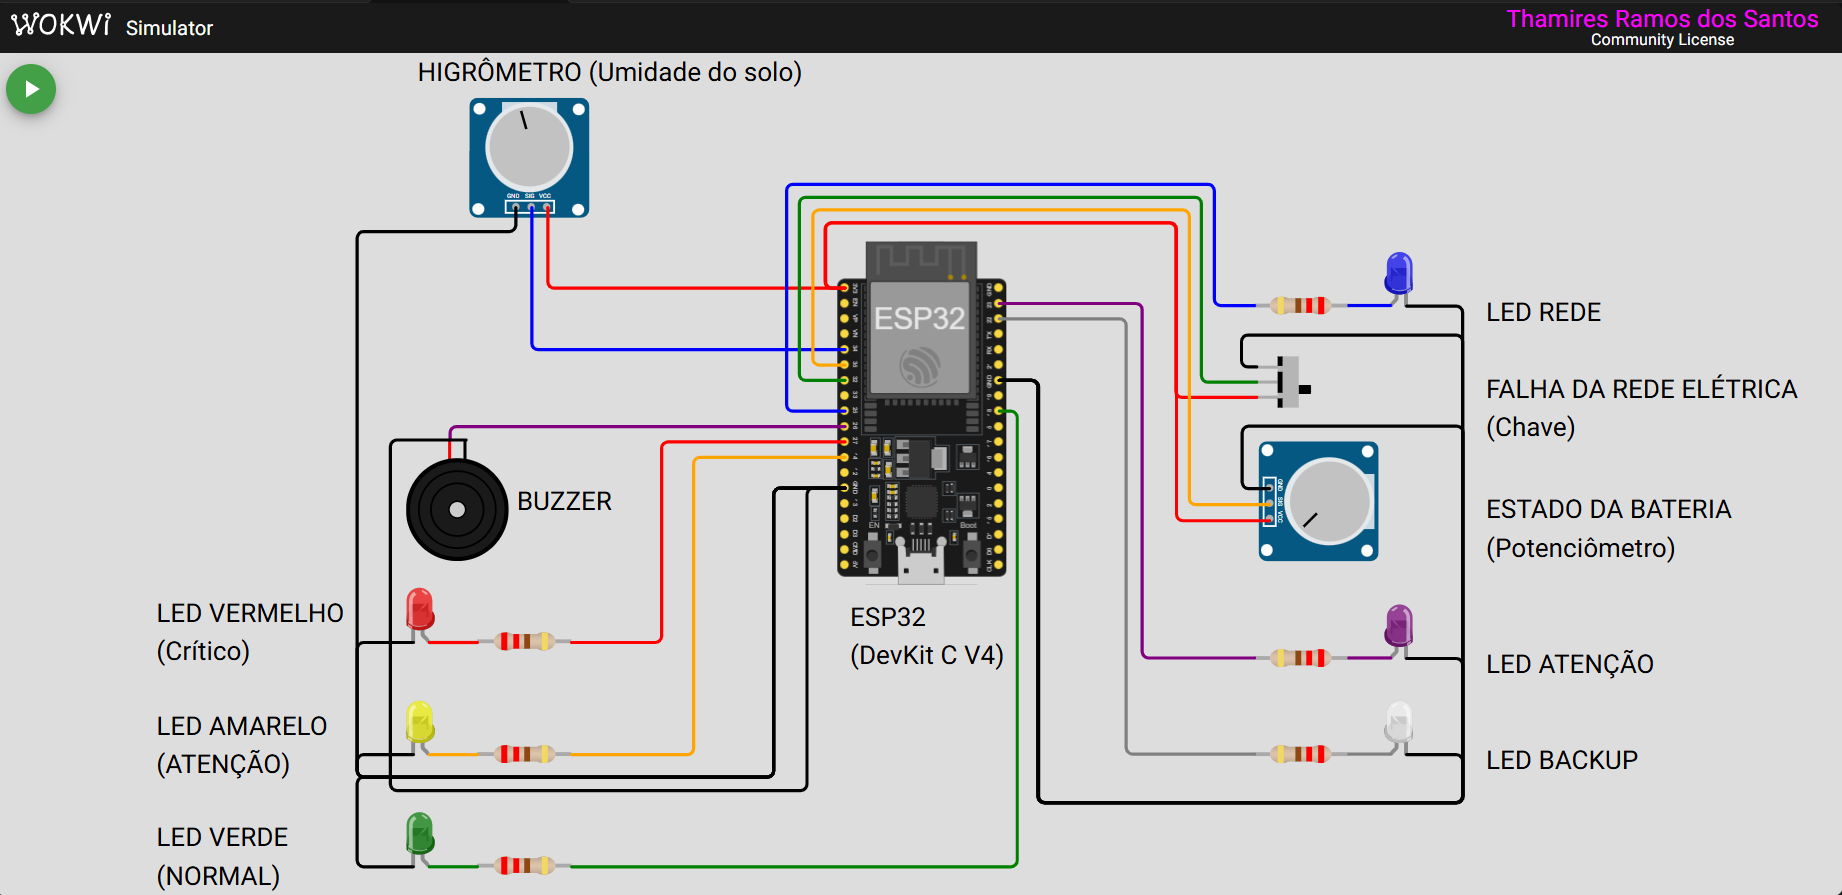
\includegraphics[width=0.9\textwidth]{figures/cap4_wokwi_circuito_v3.png}}
\caption{Circuito do ambiente de simulação Wokwi}
\label{fig:wokwi_diagrama}
\fonte{Autora, 2026.}
\end{figure}

\begin{table}[H]
\centering
\caption{Componentes do circuito virtual e o que representam}
\label{tab:componentes-wokwi}
\small
\begin{tabular}{p{4.2cm}p{0.8cm}p{1.3cm}p{8.0cm}}
\hline
\textbf{Componente} & \textbf{Qtd.} & \textbf{Pino} & \textbf{O que representa} \\
\hline
ESP32 DevKit C V4 & 1 & -- & ESP8266 NodeMCU do protótipo físico \\
Potenciômetro (solo) & 1 & GPIO34 & Higrômetro; a leitura do conversor entra na \autoref{eq:saturacao} \\
LED verde, amarelo e vermelho & 3 & GPIO18, 14, 27 & LEDs de nível de alerta (no protótipo físico, o nível VERDE usa LED azul) \\
\textit{Buzzer} & 1 & GPIO26 & \textit{Buzzer} ativo TMB-12A03, acionado no VERMELHO \\
Chave deslizante & 1 & GPIO32 & Presença da rede elétrica (saída PG do carregador): nível alto, rede presente; nível baixo, falta de rede \\
Potenciômetro (bateria) & 1 & GPIO35 & Tensão da bateria, de 2,50 a 4,20\,V \\
LED REDE (azul) & 1 & GPIO25 & Alimentação pela rede elétrica \\
LED BACKUP (branco) & 1 & GPIO22 & Alimentação pela bateria \\
LED ATENÇÃO (roxo) & 1 & GPIO23 & Bateria baixa, crítica ou com falha (\autoref{tab:estados-energia}) \\
Resistor de 220\,$\Omega$ & 6 & -- & Limitação de corrente dos LEDs virtuais \\
\hline
\end{tabular}
\fonte{Elaborado pela autora com base no arquivo \texttt{diagram.json} do projeto e em \citeonline{espressif_esp32,wokwi_potentiometer,wokwi_slideswitch,wokwi_buzzer}.}
\end{table}

O potenciômetro do solo fornece ao conversor de 12 \textit{bits} do ESP32
valores de 0 a 4095 \cite{espressif_esp32}. Esse valor substitui a leitura
do higrômetro na \autoref{eq:saturacao}, com a mesma calibração por solo
seco e solo saturado.

As leituras nos extremos da escala (0 ou 4095) são tratadas como falha do
higrômetro, pois correspondem a circuito aberto ou em curto. Assim, as
regras de contingência da \autoref{tab:contingencia} também podem ser
testadas.

O potenciômetro da bateria é convertido linearmente em tensão, de 2,50\,V
no início do curso a 4,20\,V no fim. Esses extremos são a tensão de corte
e a tensão de fim de carga da NCR18650B \cite{panasonic_ncr18650b}. A
chave e o potenciômetro alimentam os estados da \autoref{tab:estados-energia}.

O \textit{buzzer} do Wokwi é piezoelétrico e emite som apenas com sinal
oscilante \cite{wokwi_buzzer}. Para reproduzir o \textit{buzzer} ativo,
o \textit{firmware} da simulação gera, no nível VERMELHO, um sinal de
2300\,Hz, frequência de ressonância do TMB-12A03 \cite{quickteck_tmb12a03}.

Os LEDs virtuais foram ligados com resistor em série, ao contrário dos
LEDs do protótipo físico. O simulador não reproduz o consumo de energia;
por isso, nenhum valor de corrente foi obtido da simulação, e o consumo
foi calculado a partir dos \textit{datasheets} (\autoref{tab:consumo}).

Para os testes, o \textit{firmware} da simulação possui um modo de
demonstração que divide todos os tempos por 120. Os intervalos de 60 e
10~minutos passam a 30 e 5~segundos, e o tempo $T_{\mathrm{carga}}$
(\autoref{eq:tempo-carga}), de 19,5\,h, passa a 585~segundos.

O \textit{firmware} também aceita comandos pelo monitor serial, usados
apenas em teste. O comando \texttt{chuva <mm>} substitui $P_{72}$ por um
valor informado, e \texttt{chuva na} simula as APIs indisponíveis.

O comando \texttt{chuva parcial <mm>} simula dados de chuva incompletos:
um dos dias de $P_{48,\mathrm{obs}}$ fica sem registro, e o valor
informado passa a ser o mínimo garantido de $P_{72}$
(\autoref{subsec:contingencia}). Os
comandos \texttt{status} e \texttt{calibrar} mostram as leituras e gravam
a calibração do solo.

% =============================================================
\section{Testes de Validação}
\label{sec:testes-validacao}
% =============================================================

A validação foi feita por casos de teste executados na simulação
(\autoref{subsec:wokwi}). Cada caso define uma condição de entrada e a
saída esperada, obtida das regras do modelo de alerta
(\autoref{sec:modelo-risco}) e dos estados de energia
(\autoref{tab:estados-energia}).

Em cada caso, foram registrados o circuito virtual, com os LEDs, e o
monitor serial, com a leitura do solo, a chuva, o nível, a energia e o
objeto JSON enviado ao \textit{backend}. A chegada dos dados foi conferida
no painel do administrador. Os resultados são apresentados no
\autoref{cap:resultados}.

Os casos foram organizados em três grupos: os nove casos do modelo de
alerta (\autoref{tab:casos-modelo}), os casos de contingência
(\autoref{tab:casos-contingencia}) e os casos de energia
(\autoref{tab:casos-energia}). Um quarto grupo de casos foi executado no
protótipo físico (\autoref{tab:casos-fisico}).

\paragraph*{Casos do modelo de alerta}

Os nove casos combinam três valores de $S$ com três valores de $P_{72}$,
um em cada faixa da \autoref{tab:limiares}. Os valores foram escolhidos
longe dos limiares, para que o resultado não dependa do ajuste fino do
potenciômetro.

O valor de $S$ foi ajustado no potenciômetro do solo, e o de $P_{72}$ foi
informado pelo comando \texttt{chuva <mm>}. Nesses casos, a rede elétrica
permaneceu presente e a bateria em 4,20\,V. A saída esperada segue a
\autoref{tab:matriz}.

\begin{table}[H]
\centering
\caption{Casos de teste do modelo de alerta}
\label{tab:casos-modelo}
\small
\begin{tabular}{p{1.0cm}p{3.5cm}p{1.5cm}p{8.4cm}}
\hline
\textbf{Caso} & \textbf{$S$} & \textbf{$P_{72}$ (mm)} & \textbf{Saída esperada} \\
\hline
C01 & 0,40 ($S < S_1$) & 30 & VERDE; LED verde; \textit{buzzer} desligado \\
C02 & 0,40 ($S < S_1$) & 80 & VERDE; LED verde; \textit{buzzer} desligado \\
C03 & 0,40 ($S < S_1$) & 120 & VERDE; LED verde; \textit{buzzer} desligado \\
C04 & 0,75 ($S_1 \leq S < S_2$) & 30 & VERDE; LED verde; \textit{buzzer} desligado \\
C05 & 0,75 ($S_1 \leq S < S_2$) & 80 & AMARELO; LED amarelo; \textit{buzzer} desligado \\
C06 & 0,75 ($S_1 \leq S < S_2$) & 120 & AMARELO; LED amarelo; \textit{buzzer} desligado \\
C07 & 0,95 ($S \geq S_2$) & 30 & VERDE; LED verde; \textit{buzzer} desligado \\
C08 & 0,95 ($S \geq S_2$) & 80 & AMARELO; LED amarelo; \textit{buzzer} desligado \\
C09 & 0,95 ($S \geq S_2$) & 120 & VERMELHO; LED vermelho; \textit{buzzer} acionado \\
\hline
\end{tabular}
\fonte{Elaborado pela autora com base na \autoref{tab:matriz}.}
\end{table}

Os casos C03 e C07 verificam que a chuva sem solo úmido, e o solo úmido
sem chuva, não elevam o nível. Os casos C06 e C09 têm a mesma chuva e
diferem apenas em $S$.

\paragraph*{Casos de contingência}

Os casos de contingência verificam as regras da
\autoref{tab:contingencia}. A falha do higrômetro foi representada pelo
potenciômetro do solo no início do curso, e a falta de dados de chuva,
pelo comando \texttt{chuva na}. O caso X06 combina as duas falhas.

O caso X05 usou as APIs reais, sem valor informado. Nele, os dados de
chuva podem estar completos ou incompletos, quando uma das APIs falha ou
um dos dias não tem registro na estação (\autoref{subsec:bndmet}). Nesse
último caso, o nível é avaliado com o mínimo garantido de $P_{72}$
(\autoref{subsec:contingencia}).

Como a ocorrência de dados incompletos nas APIs reais não pode ser
controlada, os casos X07 a X09 a reproduzem pelo comando
\texttt{chuva parcial <mm>}. O caso X09 verifica que um mínimo garantido
abaixo de $P_1$ é tratado como falta de dados de chuva.

\begin{table}[H]
\centering
\caption{Casos de teste de contingência e de integração com as APIs}
\label{tab:casos-contingencia}
\small
\begin{tabular}{p{0.8cm}p{6.3cm}p{7.6cm}}
\hline
\textbf{Caso} & \textbf{Condição de entrada} & \textbf{Saída esperada} \\
\hline
X01 & Higrômetro indisponível; $P_{72} = 80$\,mm & AMARELO, pela chuva; aviso de higrômetro indisponível \\
X02 & Higrômetro indisponível; $P_{72} = 120$\,mm & VERMELHO, pela chuva; \textit{buzzer} acionado; aviso de higrômetro indisponível \\
X03 & $S = 0{,}95$; sem dados de chuva & AMARELO (caso especial); aviso ``sem dados de chuva'' \\
X04 & $S = 0{,}75$; sem dados de chuva & VERDE; aviso ``sem dados de chuva'' \\
X05 & APIs reais (BNDMET e OpenWeatherMap) & $P_{48}$, $P_{24}$ e $P_{72}$ do dia da consulta; com dados incompletos, aviso ``dados de chuva incompletos'' e nível avaliado com o mínimo garantido de $P_{72}$; sem nenhuma parcela, aviso ``sem dados de chuva'' \\
X06 & Higrômetro indisponível; sem dados de chuva & AMARELO (regra de precaução); avisos de higrômetro indisponível e ``sem dados de chuva'' \\
X07 & $S = 0{,}95$; dados de chuva incompletos, mínimo garantido de 120\,mm & VERMELHO, avaliado com o mínimo garantido; \textit{buzzer} acionado; aviso ``dados de chuva incompletos'' \\
X08 & $S = 0{,}75$; dados de chuva incompletos, mínimo garantido de 80\,mm & AMARELO, avaliado com o mínimo garantido; aviso ``dados de chuva incompletos'' \\
X09 & $S = 0{,}95$; dados de chuva incompletos, mínimo garantido de 30\,mm & AMARELO (caso especial), pois o mínimo é menor que $P_1$; aviso ``dados de chuva incompletos'' \\
\hline
\end{tabular}
\fonte{Elaborado pela autora com base na \autoref{tab:contingencia}.}
\end{table}

\paragraph*{Casos de energia}

Os casos de energia usaram a chave da rede e o potenciômetro da bateria,
com o nível de alerta fixo em VERDE ($S = 0{,}40$ e $P_{72} = 30$\,mm). As
tensões de 3,15\,V e 2,80\,V foram escolhidas dentro das faixas de bateria
baixa e crítica da \autoref{tab:estados-energia}.

No caso E04, a bateria foi mantida abaixo de 4,20\,V com a rede presente
até o fim do tempo $T_{\mathrm{carga}}$, reduzido a 585~segundos pelo modo
de demonstração.

\begin{table}[H]
\centering
\caption{Casos de teste da supervisão de energia}
\label{tab:casos-energia}
\small
\begin{tabular}{p{0.8cm}p{6.0cm}p{7.6cm}}
\hline
\textbf{Caso} & \textbf{Condição de entrada} & \textbf{Saída esperada} \\
\hline
E01 & Rede presente; bateria em 4,20\,V & LED REDE aceso; estado da bateria normal \\
E02 & Rede ausente; bateria em 4,20\,V & LED BACKUP aceso; aviso de falta de rede; nível de alerta mantido \\
E03 & Rede ausente; bateria em 3,15\,V e depois em 2,80\,V & LED ATENÇÃO piscando; bateria baixa e, depois, bateria crítica \\
E04 & Rede presente; bateria em 3,80\,V até o fim de $T_{\mathrm{carga}}$ & Durante a recarga, estado normal, com indicação de recarga; após $T_{\mathrm{carga}}$, LED ATENÇÃO aceso e falha de bateria, sem a indicação de recarga \\
\hline
\end{tabular}
\fonte{Elaborado pela autora com base na \autoref{tab:estados-energia}.}
\end{table}

Os valores de $S$ e de tensão desses casos vêm dos potenciômetros da
simulação e não são medições. O objetivo dos casos é verificar a lógica
de decisão do \textit{firmware}, e não o comportamento do solo ou da
bateria.

\paragraph*{Casos no protótipo físico}

O protótipo físico executa a mesma lógica de alerta da simulação, com o
higrômetro real no lugar do potenciômetro e sem a supervisão de energia
(\autoref{subsec:arquitetura}). Os casos da \autoref{tab:casos-fisico}
verificam a leitura do higrômetro, a decisão do nível e o acionamento dos
LEDs e do \textit{buzzer} reais.

Antes dos casos, o higrômetro foi calibrado com a sonda em solo seco e com
a sonda imersa em água, pelo comando \texttt{calibrar}. A saturação $S$ de
cada caso foi obtida variando a umidade do solo em torno da sonda, e
$P_{72}$ foi informado pelo comando \texttt{chuva <mm>}, como na simulação.

Como a umidade do solo não pode ser ajustada com precisão, a saída
esperada de cada caso é definida pela faixa de $S$ efetivamente lida
(\autoref{tab:limiares}), e não por um valor fixo.

\begin{table}[H]
\centering
\caption{Casos de teste no protótipo físico}
\label{tab:casos-fisico}
\small
\begin{tabular}{p{0.8cm}p{6.2cm}p{7.2cm}}
\hline
\textbf{Caso} & \textbf{Condição de entrada} & \textbf{Saída esperada} \\
\hline
F01 & Sonda em solo seco ($S < S_1$); $P_{72} = 120$\,mm & VERDE; LED azul; \textit{buzzer} desligado \\
F02 & Sonda em solo úmido ($S_1 \leq S < S_2$); $P_{72} = 80$\,mm & AMARELO; LED amarelo; \textit{buzzer} desligado \\
F03 & Sonda em solo saturado ($S \geq S_2$); $P_{72} = 120$\,mm & VERMELHO; LED vermelho; \textit{buzzer} acionado \\
F04 & Sonda em solo saturado ($S \geq S_2$); $P_{72} = 30$\,mm & VERDE; LED azul; \textit{buzzer} desligado \\
F05 & Sonda desconectada do módulo; $P_{72} = 80$\,mm & AMARELO, pela chuva; aviso de higrômetro indisponível \\
F06 & Sonda em solo saturado ($S \geq S_2$); sem dados de chuva & AMARELO (caso especial); aviso ``sem dados de chuva'' \\
F07 & APIs reais (BNDMET e OpenWeatherMap) & $P_{48}$, $P_{24}$ e $P_{72}$ do dia da consulta; com dados incompletos, aviso ``dados de chuva incompletos'' e nível avaliado com o mínimo garantido; sem nenhuma parcela, aviso ``sem dados de chuva'' \\
F08 & Sonda em solo saturado ($S \geq S_2$); dados de chuva incompletos, mínimo garantido de 120\,mm & VERMELHO, avaliado com o mínimo garantido; LED vermelho; \textit{buzzer} acionado \\
\hline
\end{tabular}
\fonte{Elaborado pela autora com base nas \autoref{tab:matriz} e \autoref{tab:contingencia}.}
\end{table}

No protótipo físico, $S$ vem do higrômetro, mas os casos continuam sendo
testes da lógica de decisão: a umidade do solo em torno da sonda foi
preparada para cada caso e não representa o maciço de uma barragem.